\chapter{Methodology}
\label{ch:methodology}

This chapter will address the core contributions of our project.
We present the hardware involved in \gls{sensorfusion}, describe the data acquisition procedure, then introduce our final solution, by detailing the research and implementation process, as well as design decisions that had to be made along the way.

\section{Prerequisites}

\newcommand{\wvec}{\vecx{w}}
\newcommand{\what}{\widehat{\vecx{w}}}
\newcommand{\wmod}{\left|\vecx{w}\right|}
\newcommand{\xihat}{\widehat{\xi}}

Let us first introduce the mathematical notions used throughout this work. The group of rotations in 3D space is $\SO{3} = \left\{\matx{R} \in \RR^{3\times3} : \det{\matx{R}} = 1, \transpose{\matx{R}}\matx{R} = \matx{I}_3 \right\}$. For any vector $\wvec \in \RR^3$ we can define a \emph{skew-symmetric} matrix:
\begin{equation}
	\what  = \skewsym{\wvec} =
	\begin{bmatrix}
		0    & -w_3 & w_2  \\
		w_3  & 0    & -w_1 \\
		-w_2 & w_1  & 0
	\end{bmatrix}
\end{equation}
and $\so{3} = \left\{\what : \vecx{w} \in \RR^3 \right\}$ is the set of all such matrices.
The exponential maps \mbox{$\text{exp}:\so{3} \rightarrow \SO{3}$} and \mbox{$\text{Exp} :\RR^3 \rightarrow \SO{3}$} are defined as
\mbox{$\expmap{\what} =\Expmap{\wvec}= e^{\what}$}, and Rodrigues' formula \cite{murray2017mathematical} provides a closed formulation of the matrix exponential:
\begin{equation}
	e^{\what}= \matx{I}_3 + \frac{\what}{\wmod} \sin{\wmod} + \frac{\what^2}{\wmod^2}\left(1 - \cos{\wmod}\right)\eqdot
\end{equation}
The inverse operations are $\text{log}:  \SO{3} \rightarrow \so{3}$ and $\text{Log} :\SO{3} \rightarrow \RR^3$, respectively. If $\what = \logmap{\matx{R}}$ and $\matx{R} \neq \matx{I}_3$, then:
\begin{equation}
	\wmod = \cos^{-1}\left(\frac{\text{tr}(\matx{R}) - 1}{2}\right)
	\text{ and }
	\frac{\wvec}{\wmod} = \frac{1}{2\sin{\wmod}}\begin{bmatrix}
		r_{32} - r_{23} \\ r_{13} - r_{31} \\ r_{21}-r_{12}
	\end{bmatrix}
	\comma
\end{equation}
and if $\matx{R} = \matx{I}_3$, $\wmod=0$.

Furthermore, we consider the group of Euclidean transformations in 3D space (rotation and translation):
\begin{equation}
	\SE{3}= \left\{
	\Mtx{} \in \RR^{4\times4} : \Mtx{} =
	\begin{bmatrix}
		\matx{R} & \vecx{t} \\ \transpose{\vecx{0}} & 1
	\end{bmatrix}, \matx{R} \in \SO{3}, \vecx{t} \in \RR^3
	\right\}\eqdot
\end{equation}

The corresponding tangent space is:
\begin{equation}
	\se{3} = \left\{
	\xihat \in \RR^{4\times4} : \xihat =
	\widehat{\begin{bmatrix}
			\vecx{v} \\ \wvec
		\end{bmatrix}} = \begin{bmatrix}
		\what                & \vecx{v} \\
		\transpose{\vecx{0}} & 1
	\end{bmatrix}, \wvec \in \RR^3, \vecx{v} \in \RR^3
	\right\}\eqdot
\end{equation}

The exponential maps $\text{exp}: \se{3} \rightarrow \SE{3}$ and $\text{Exp} :\RR^6 \rightarrow \SE{3}$ are defined as:
\begin{equation}
	\expmap{\xihat} = \Expmap{\xi} = \begin{bmatrix}
		\Expmap{\wvec}       & \matx{V}(\wvec)\vecx{v} \\
		\transpose{\vecx{0}} & 1
	\end{bmatrix}\comma
\end{equation}
where:
\begin{equation}
	\matx{V}(\vecx{w}) = \matx{V}(\theta\vecx{u})  = \matx{I}_3 + \frac{1-\cos\theta}{\theta}\widehat{\vecx{u}} + \frac{\theta-\sin\theta}{\theta}\widehat{\vecx{u}}^2\eqdot
\end{equation}

The logarithmic map $\text{Log} :\SE{3} \rightarrow \RR^6$ is:
\begin{equation}
	\xi = \Logmap{\begin{bmatrix}
			\matx{R} & \vecx{t} \\ \transpose{\vecx{0}} & 1
		\end{bmatrix}} = \begin{bmatrix}
		\matx{V}^{-1}(\vecx{w}) \vecx{t} \\
		\Logmap{\matx{R}}
	\end{bmatrix}\comma
\end{equation}
and we express $\text{log} :\SE{3} \rightarrow \se{3}$ as $\xihat = \logmap{\Mtx{}} = \widehat{\Logmap{\Mtx{}}}$. This allows introducing an interpolation function, with a parameter $\alpha \in \left[0, 1\right]$:
\begin{equation}
	\label{eq:se3-interpolation}
	\varphi\left(\Mtx{1}, \Mtx{2}, \alpha\right) :=
	\Mtx{1} \expmap{\alpha \cdot \logmap{\Mtx{1}^{-1} \Mtx{2}}}
	\eqdot
\end{equation}
\section{Hardware}

In this context, hardware refers to the set of sensors used for data collection, determined by the existing industrial setup. The data capturing system is controlled by an Nvidia Jetson board, which operates as a middle-man for time synchronisation between the sensors, and coordinates the various data streams. Even though the solution was designed such that it does not inherently rely on any particular device, the relationship between hardware capabilities, data quality and final output makes it crucial to understand the sensors involved in the process. Beyond the components described below, the setup includes three industrial grade ArkCam Basic+ wide angle cameras which provide a 1920x1080 RGB stream over Ethernet. These are not utilised within this project, but represent a noticeable motivation for future work directions.

\begin{figure}
	\centering
	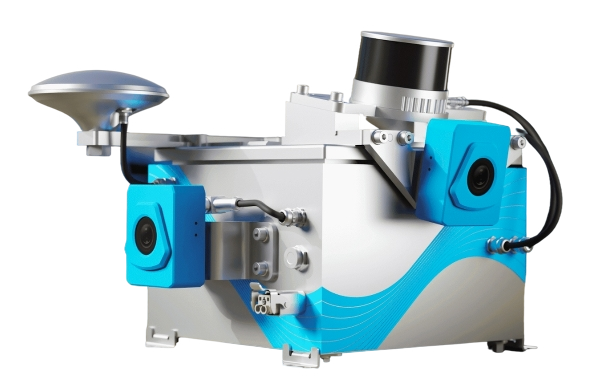
\includegraphics[width=0.6\linewidth]{images/sdx-compact-on-top-nobg.png}
	\caption[SDX-Compact]{The SDX-Compact manufactured by Sodex Innovations GmbH. The set of sensors consists of a 3D LiDAR scanner, three RGB cameras and a high-accuracy positioning system. Image source: \href{https://www.geo-lanes.com/sodex-innovations/}{GeoLanes}}
	\label{fig:sdx-compact}
\end{figure}

\subsection{LiDAR Sensor}

The SDX-Compact \reffigbr{sdx-compact} is equipped with a Pandar XT32 \cite{hesai_xt16_32_32m} LiDAR sensor, manufactured by Hesai Technology. This is a mechanical rotating LiDAR with a full $360 \degree$ horizontal field of view and 32 beams distributed vertically, at $1 \degree$ resolution. With our settings, the sensor produces 10 complete scans per second, resulting in a horizontal resolution of $0.18 \degree$. The maximum operational range is 120m, decreasing to 50m for low-reflectivity targets. The official specifications state a typical accuracy of $\pm 1$cm, with precision $\pm 0.5$cm, in a static environment. For each beam, the strongest return is processed, leading to 640,000 points being generated per second. The high output bandwidth is handled by an Ethernet connection, over which points are sent as \acrshort{udp} packets. The sensor also supports \acrshort{ptp} synchronisation, essential for high-quality sensor fusion.

The same device has been used for LiDAR odometry applications in the past \cite{kicp}, and has similar specifications to other popular scanners, such as Velodyne VLP-32C, Ouster OS1-32 or Robosense Helios 32.

\subsection{GNSS/INS receiver}

Another component of the sensor stack is the Septentrio AsteRx SBi3 Pro+ GNSS/INS receiver \cite{Septentrio_AsteRx_SBi3_Pro+}, which provides global positioning and orientation data at a rate of 100Hz. Internally, this relies on two distinct mechanisms.

The localization information comes from a dual antenna GNSS module compatible with several GNSS consellations (\eg \acrshort{gps}\footnote{Throughout this paper, GNSS and GPS are used interchangeably to refer to the global localization sensor, regardless of the underlying satellite system used during data collection.}, \acrshort{glonass}, Galileo), to ensure optimal worldwide coverage. In standalone mode, the advertised typical accuracy is 1m, but the receiver also acts as an NTRIP (a protocol for differential GPS) client, gathering correction information, in order to achieve centimeter-level accuracy.

An \acrfull{imu} module records acceleration data and provides the remaining orientation angles (roll, pitch, yaw) to compute the complete pose, in 6 \acrfull{dof}. This is integrated with the absolute GNSS measurements using the patented FUSE+ technology \cite{Septentrio_FUSE_Sensor_Fusion}, resulting in an orientation error below  $\text{5-10}\degree$.

Like any system reliant on satellite communication, this will suffer significantly in situations where the signal propagation is disturbed (heavy clouds, ``urban canyons'', thick vegetation, spoofing), even leading to loss of \emph{\gls{gnssfix}}.

To conclude this section, we recognize and underline the importance of accurate extrinsic calibration between the LiDAR and the local INS coordinate frame, which has to be performed prior to any reliable data collection procedure. Given the radically different modalities of these two sensors, this is not a trivial task \cite{lidar-gps-calib} and lies outside the scope of the current work.

\begin{figure}
	\centering
	\subcaptionbox{The trajectory, overlaid on a satellite image of the region.}{
		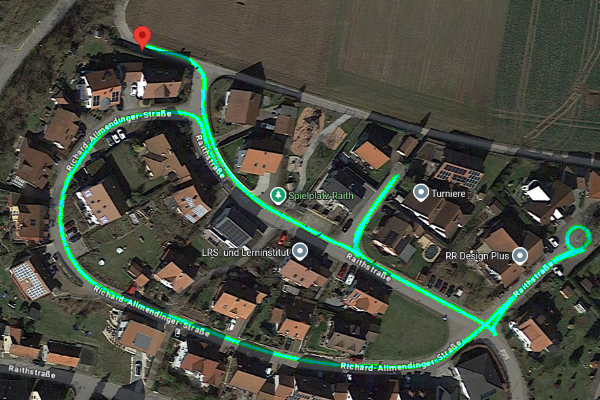
\includegraphics[width=0.45\linewidth]{images/example-trajectory.png}}
	\hspace{1pt}
	\subcaptionbox{Standard deviation of GNSS readings along the trajectory.}{
		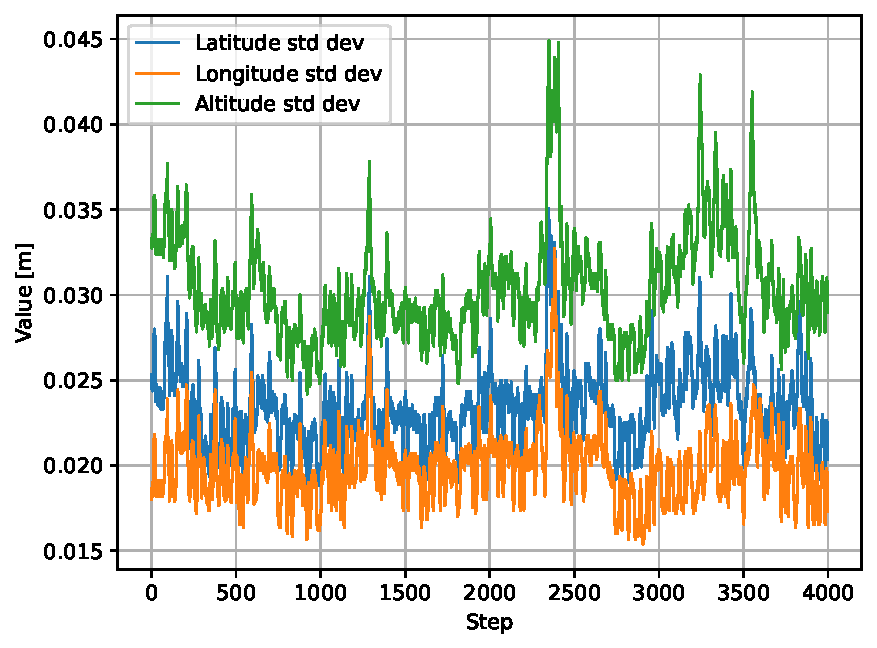
\includegraphics[width=0.45\linewidth]{images/example-trajectory-sigma.pdf}}
	\caption[Example dataset trajectory]{An example dataset collected in rural Germany (Lienziegen).}
	\label{fig:example-trajectory}
\end{figure}

% 48.97905882 lat
% 8.86602707 lon

\section{Data acquisition and pre-processing}
\label{sec:data-acquisition}

Data is collected by mounting the sensor rig on the roof of a vehicle, and driving around a target area at a relatively low speed (\eg up to 40km/h), see Fig.~\ref{fig:example-trajectory}. In comparison with other public datasets \cite{nuscenes, pixset}, capturing data in non-urban environments introduces some challenges --- scenes dominated by vegetation, with few identifiable features, uneven terrain --- while minimizing others --- negligible amount of dynamic objects, no tall buildings that could affect GNSS signal propagation.

The raw sensor output is uploaded to a cloud storage facility, and is later processed into \emph{data frames} that fuse the available information \reffigbr{data-sync}. This can occur because the sensors are PTP-synchronized on initialization, and all recorded data is timestamped.


\begin{figure}
	\centering
	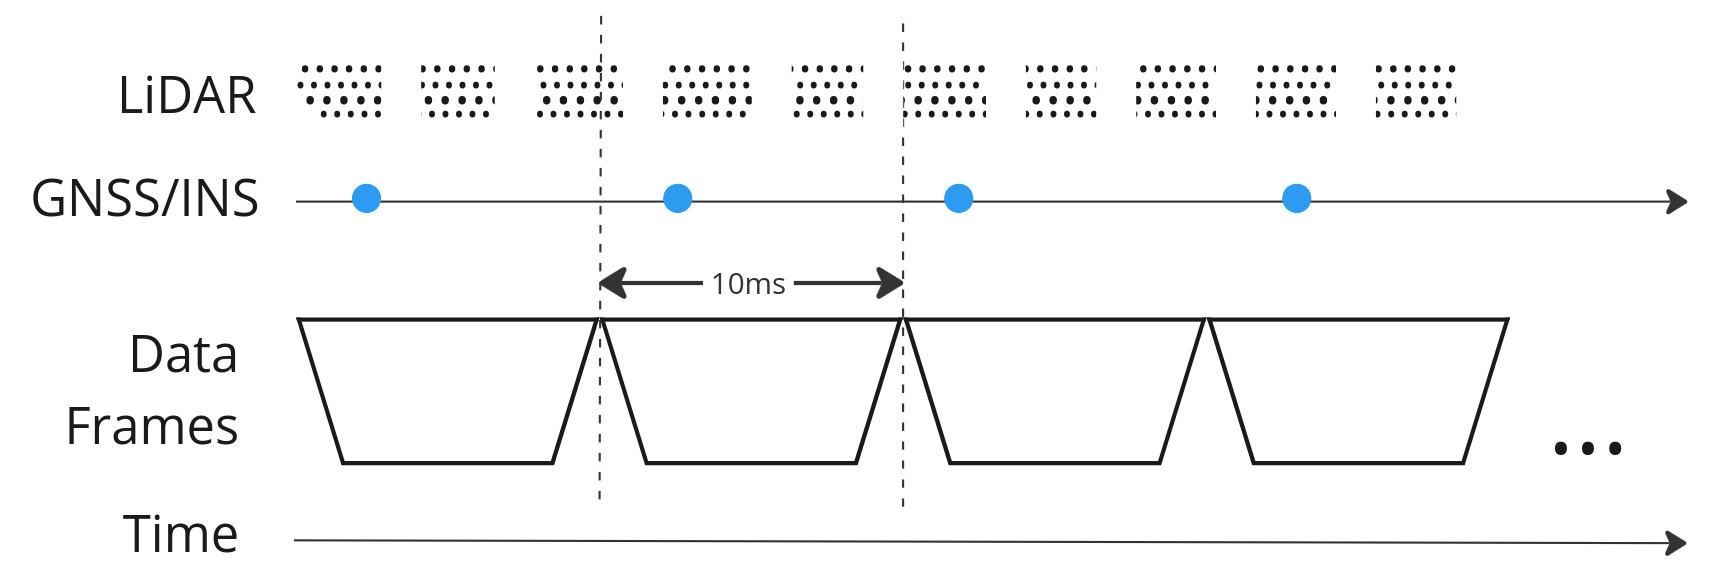
\includegraphics[width=0.7\linewidth]{images/data_sync.jpg}
	\caption[Data frame synchronisation]{The data synchronisation process.\\Time is discretized into fixed-size intervals, resulting in data frames of custom resolution. These are populated with information from the two sensors: LiDAR points arrive in groups, as UDP packets, while GNSS readings have a frequency of approx. 100Hz. We employ a data frame size of 10ms to ensure that each interval has an associated GNSS measurement, and place all corresponding packets in the same data frame.}
	\label{fig:data-sync}
\end{figure}

The next pre-processing step consists of dividing the sequence of data frames such that we operate on individual scans (also known as sweeps) produced by the LiDAR. A scan corresponds to a complete $360 \degree$ rotation, which takes 100ms, so we join the points in 10 consecutive data frames to obtain a single scan.

Every INS reading undergoes a map projection, to obtain $x,y,z$ coordinates in the East-North-Up frame. We consider the frame of the GNSS receiver as the $ego$ coordinate system. The roll $\phi$, pitch $\theta$ and yaw angles $\psi$ determine the absolute orientation, so we compute a global pose $\egoposet{} \in \SE{3}$ as:

\begin{equation}
	\egoposet{} =
	\text{Translation}(x, y, z) \cdot
	\rotmtx{z}{\psi} \cdot
	\rotmtx{x}{\theta} \cdot
	\rotmtx{y}{\phi}\comma
\end{equation}
where $\text{Rot}_k(\alpha)$ is the transformation matrix corresponding to a rotation of $\alpha$ around axis $k$.
Because the sensor provides error estimates in the form of global one-sigma values $\left\{ \sigma_x, \sigma_y, \sigma_z, \sigma_\phi, \sigma_\theta, \sigma_\psi\right\}$, we construct the covariance matrix:
\begin{equation}
	\matx{\Sigma} = \text{diag}\left(\varx{x}, \varx{y}, \varx{z}, \varx{\phi}, \varx{\theta}, \varx{\psi}\right)
\end{equation}
and transform it using the adjoint map of the rotation component:
\begin{equation}
	\matx{\Sigma}_{ego} =
	\adjoint{\matx{R}}{\vecx{0}} \cdot
	\matx{\Sigma} \cdot
	\transpose{\adjoint{\matx{R}}{\vecx{0}}}
	\comma
\end{equation}
where:
\begin{equation}
	\adjoint{\matx{R}}{\vecx{t}} =
	\begin{bmatrix}
		\matx{R}                   & \vecx{0}_{3\times3} \\
		\skewsym{\vecx{t}}\matx{R} & \matx{R}
	\end{bmatrix}\eqdot
\end{equation}

A LiDAR range reading $r$, captured at azimuth $\alpha$ with an elevation angle of $\phi$, can be converted to a 3D location in the LiDAR frame:

\begin{equation}
	\lidarframe{\vecx{p}}= \begin{bmatrix}
		p_x \\ p_y \\ p_z
	\end{bmatrix}=\begin{bmatrix}
		r \cos{\phi} \sin{\alpha} \\ r \cos{\phi} \cos{\alpha} \\ r \sin{\phi}
	\end{bmatrix}\eqdot
\end{equation}

If $\lidartoego$ is the pose of the LiDAR in the ego frame (from extrinsic calibration), we can compute the location of a point in the ego frame:

\begin{equation}
	\begin{bmatrix}
		{}^{ego}\vecx{p}_\lidartxt \\ 1
	\end{bmatrix}
	= \lidartoego \begin{bmatrix}
		\lidarframe{\vecx{p}} \\ 1
	\end{bmatrix}\eqdot
\end{equation}



\subsection{Motion compensation}
\label{subsec:motion-compensation}

At this stage, it is worth discussing the distortion effect that occurs when a rotating LiDAR sensor is moved at a relatively high velocity. Because it operates in a relative coordinate frame and different beams of the sweep are fired at different times, the beams corresponding to azimuth $0 \degree$ will fire approximately 100ms earlier than the beams corresponding to azimuth $359 \degree$. Placing the resulting points in the same coordinate frame would lead to undesired artifacts, such as duplicate or warped structures. \reffigbr{motion-comp-pre}

\begin{figure}[h]
	\centering
	\subcaptionbox{Before: an artificial duplicate surface \label{fig:motion-comp-pre}}{
		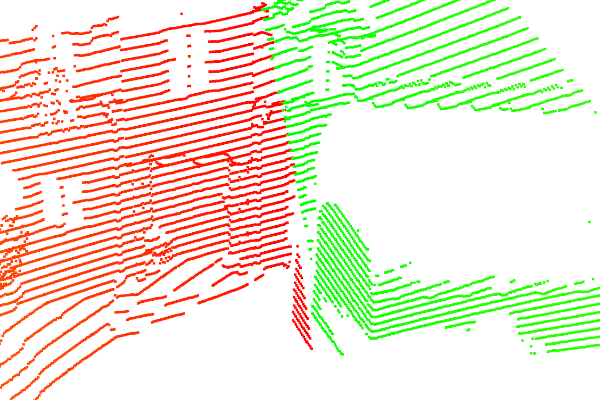
\includegraphics[width=0.45\linewidth]{images/motion-comp-pre.png}
	}
	\hspace{1pt}
	\subcaptionbox{After: surface is corrected \label{fig:motion-comp-post}}{
		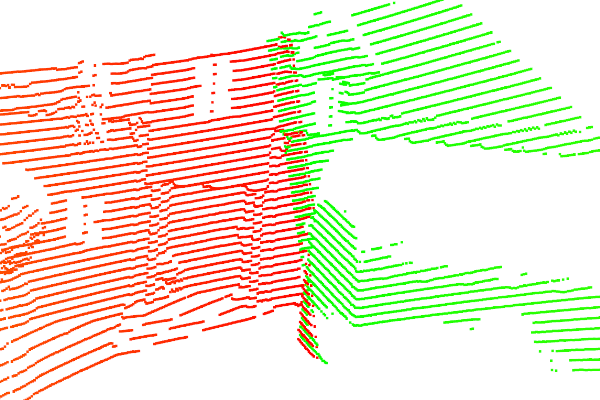
\includegraphics[width=0.45\linewidth]{images/motion-comp-post.png}
	}
	\caption[Motion compensation: before and after]{Motion artifacts and the result of motion compensation. \\Green: points from the beginning of the sweep. Red: points from the end of the sweep. Without motion compensation, the vertical surface yields two conflicting clusters, so the scan cannot be used for accurate mapping in the global frame.}
	\label{fig:motion-comp}
\end{figure}

This open research problem \cite{motion-comp-mcdermott} is commonly addressed by estimating the sensor pose change during a sweep \cite{vicp,vizzo2023ral}, and IMU integration proves satisfactory \cite{deskewing2020}, given the short time interval involved. In our case, the ego poses
$\left\{\egoposeti{i}{0}, \egoposeti{i}{1}, \dots, \egoposeti{i}{m}\right\}$
computed from INS measurements during sweep $i$ are used to bring all points into the frame defined by $\egoposeti{i}{0}$. A point $^{i,k}\vecx{p}$ belongs to data frame $k$, so it will be replaced by:

\begin{equation}
	\begin{bmatrix}
		^{i,0}\vecx{p} \\ 1
	\end{bmatrix}
	= {}^{i,0}\pose_{i,k} \begin{bmatrix}
		{}^{i,k}\vecx{p} \\ 1
	\end{bmatrix}  = \left({\egoposeti{i}{0}}\right)^{-1} \egoposeti{i}{k} \begin{bmatrix}
		{}^{i,k}\vecx{p} \\ 1
	\end{bmatrix}
	\eqdot
\end{equation}

We also experimented with approaches that do not rely on the absolute pose measurements for subsections of the sweep, such as interpolation using point timestamps or point indices (based on the order in which the points are returned), but these did not yield better results. A potential drawback of our method is that it disregards the localization noise, which could prove counterproductive if the GNSS receiver has low accuracy.

Through this step we are effectively removing the need for sub-scan information and creating a simpler data structure in which each scan is associated a single $\egoposet{}$ pose (from the first data frame), and the points in a sweep can be treated as a unified set.

Without loss of generality, we transform the sequence of global poses
$\left\{\posei{0}, \posei{1}, \dots, \posei{n}\right\}$
into the frame of the first pose, by multiplying each pose with  $\left(\posei{0}\right)^{-1}$, to obtain $\left\{\pose_0, \pose_1, \dots, \pose_n\right\}$. Naturally, $\pose_0$ will always be $\matx{I}_4$, which simplifies the initialization of the odometry estimation. The covariance of each pose is adjusted  with the adjoint of $\left(\posei{0}\right)^{-1}$.


% TODO write about projection

\section{Solution architecture}

At its core, the odometry and mapping solution that we propose requires minimal input: a sequence of point clouds captured by a moving LiDAR scanner, and a timestamp for each scan. If available, absolute localization/INS measurements can be used as additional input.

Let $\mathfrak{P} = \left\{ P_0, P_1, \dots P_n\right\}$ represent the set of point clouds that we operate on, with point coordinates $P_k = \left\{\vecx{p}_{k,i} : \vecx{p}_{k,i} \in \RR^3 \right\}$ expressed in the local frame, $\mathfrak{s} = \left\{ s_0, s_1, \dots s_n\right\}$ the corresponding timestamps, and $\widehat{\mathfrak{T}} = \left\{ \gtposei{0}, \gtposei{1}, \dots \gtposei{n} \right\}$ the ground truth poses at which each scan was captured. In an ideal setting, a point cloud registration algorithm would take $P_i$ and $P_{i+1}$ as input and return the transformation $\Delta\gtposei{i} = \gtposei{i}^{-1} \gtposei{i+1}$, \ie the ground truth displacement between consecutive poses. This would correspond to a perfect odometry model, and the complete trajectory could be reconstructed by accumulating the computed displacement. Unfortunately, with the exception of some simulation environments, such an approach is not actually feasbile. As we have already seen, LiDAR output is not perfect, especially in dynamic scenes, and some scenarios are simply unsuitable for odometry estimation based on 3D features \cite{lidartunnel}.

The output of our solution can be formulated as $\mathfrak{T} = \left\{ \pose_0, \pose_1, \dots \pose_n\right\}$. Pose \mbox{$\pose_k \in \SE{3}$} represents the estimated location and orientation of the \emph{ego} frame from which the points $P_k$ were observed. The complete \emph{map} estimate, represented as a larger point cloud in global coordinates, is the set of all points, each transformed according to their respective pose:
\begin{equation}
	M\left(\mathfrak{T}, \mathfrak{P}\right) =
	\left\{
	\vecx{p}_{k,i}^* \in \RR^3:
	\begin{bmatrix}
		\vecx{p}_{k,i}^* \\ 1
	\end{bmatrix} =
	\pose_k \begin{bmatrix}
		\vecx{p}_{k,i} \\ 1
	\end{bmatrix}, \vecx{p}_{k,i} \in P_k, k \in \overline{0 \dots n}
	\right\}\eqdot
\end{equation}

This uncovers two possible evaluation directions, which also constitute the high-level aims of our method. On one hand, the output trajectory  $\mathfrak{T}$ should match the actual path of the system as accurately as possible. On the other, the final map $M\left(\mathfrak{T}, \mathfrak{P}\right)$ should not hide or damage small details in the scene, to obtain a high-quality 3D reconstruction. Although not immediately obvious, these can result in conflicting requirements, but they anticipate an underlying optimization problem.

\begin{figure}[h]
	\centering
	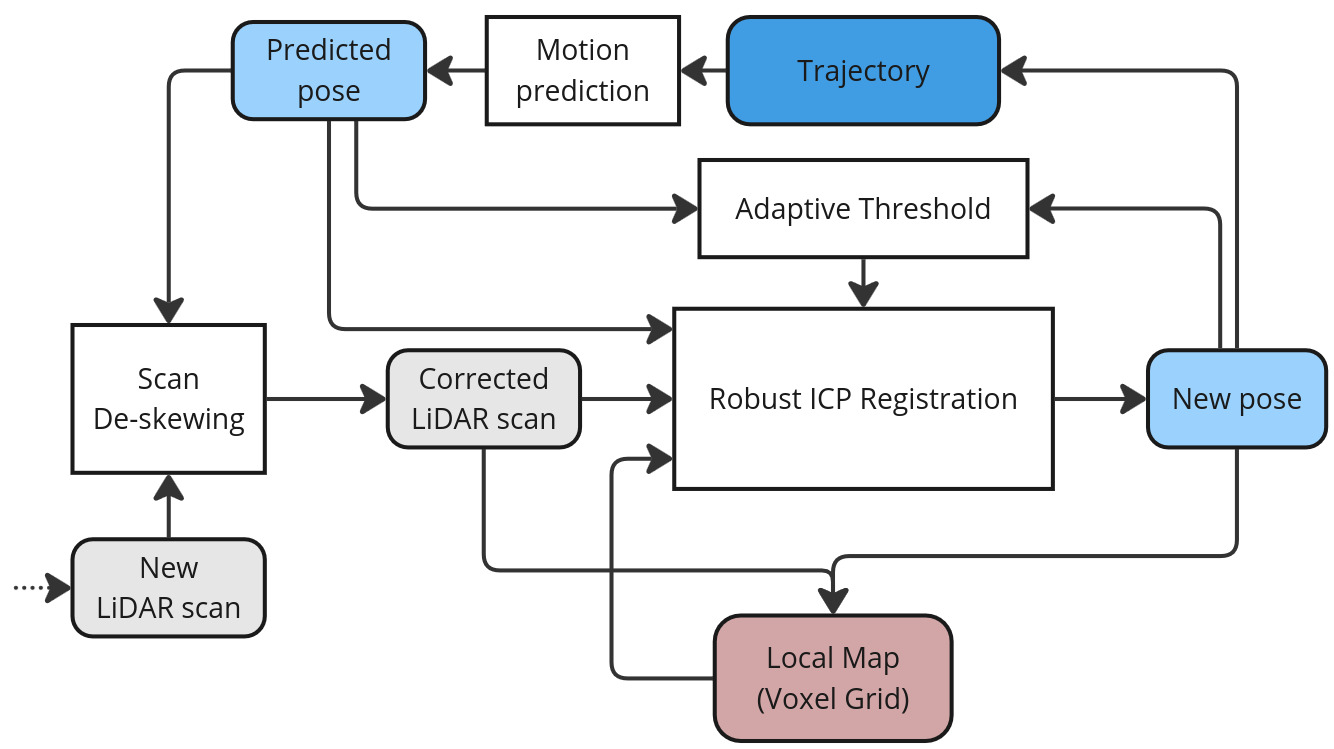
\includegraphics[width=0.6\linewidth]{images/kiss-icp-architecture.jpg}
	\caption[KISS ICP Architecture]{The KISS ICP pipeline.\\An incoming scan is motion-compensated using the displacement between the previous estimated poses, then it is downsampled and registered against the local map. The pose estimated by the ICP algorithm is added to the trajectory, and the adaptive threshold is updated by evaluating the accuracy of the motion estimation. This determines the ICP outlier removal threshold, improving the system's ability to react to unexpected motions.}
	\label{fig:kiss-icp-architecture}
\end{figure}

\subsection{Overview}

The final architecture is the result of a series of experiments. The process began with a LiDAR-only framework, immitating the KISS-ICP \cite{vizzo2023ral} implementation. \reffigbr{kiss-icp-architecture} In this approach, scans are processed one-by-one, attempting to compute the optimal pose at each step, and the map is built incrementally. This is computationally efficient and becomes essential when a robot operates in an unknown environment, as it provides a localization estimate at any given time. In the absence of absolute positioning information, however, this diverges from the ground-truth trajectory \reffigbr{deviation-no-gps}, creating a distorted map.

\begin{figure}[h]
	\centering
	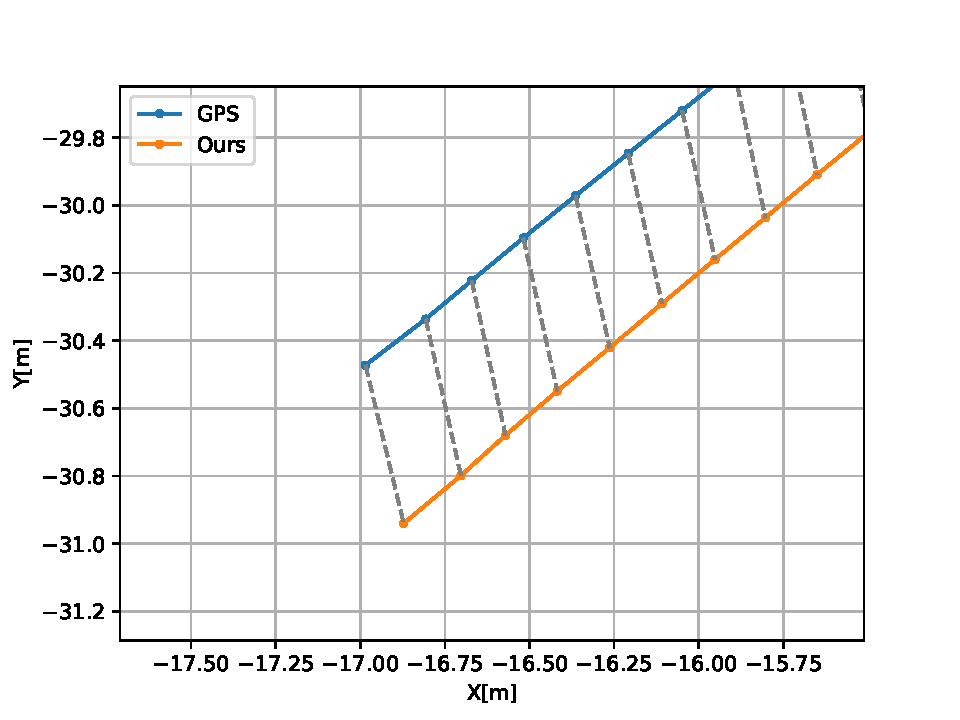
\includegraphics[width=0.5\linewidth]{images/deviation_30s.pdf}
	\caption[Trajectory deviation from GPS]{When the GPS information is not used, the trajectory computed based on LiDAR data diverges. Here, after 300 scans (approx. 30 seconds), the last location is approx. 0.5m away from the corresponding GPS position.}
	\label{fig:deviation-no-gps}
\end{figure}

Early efforts focused on introducing the GPS readings as a constraint at each step, alongside motion prediction and registration results. This led to experimenting with each component, as well as methods for combining the respective poses, while regularly monitoring the quality of the output trajectories and maps. As the solution was evolving, it was tested on more challenging scenarios, by adding artificial noise to the GPS readings, or skipping some of them altogether.

Later on, we also considered addressing the pose estimation problem holistically, instead of in an incremental fashion, and experimented with architectures based on factor graph optimization \cite{dellaert2017factor}, where nodes are linked using registration and GPS constraints. The same building blocks are needed, but the relationship between them is guided by the graph paradigm. Eventually, this was adapted to obtain a hybrid solution \reffigbr{solution-architecture}, which combines the advantages of the two frameworks in a very intuitive manner.


\subsection{Reconciling motion prediction, GNSS and registration}
\label{subsec:reconciling}
Before discussing the components in detail, we would like to provide a general picture of the rationale behind combining the pose estimates that we operate on. We assume that for every scan $P_k$ we can compute three poses in the world frame, and aim to generate $\pose_k$ as a function of these:
\newcommand{\tkicp}{\pose_k^{\text{ICP}}}
\newcommand{\tkgps}{\pose_k^{\text{GPS}}}
\newcommand{\covicp}{\matx{\Sigma}_{\text{ICP}}}
\newcommand{\covgps}{\matx{\Sigma}_{\text{GPS}}}
\begin{compactenum}
	\item A registration-predicted pose $\tkicp$, from a point cloud registration method that optimizes map alignment between scans in the global frame.
	\item An absolute localization pose $\tkgps$, generated by the INS sensor.
	\item A motion-predicted pose $\pose_k'$, output by the algorithm described in Section \ref{subsec:motion-prediction}.
\end{compactenum}

Each of these serves a different purpose: using only $\tkicp$ would lead to a high-quality 3D map, while diverging from the actual locations; $\tkgps$ estimates the absolute position and orientation, but its accuracy varies depending on the environment; the $\pose_k'$ pose can help filter out noise in the GNSS data and smoothen the trajectory, but comes from a motion prediction mechanism that cannot operate in the absence of other sensors.

In an initial trial, we observed what happens when the GPS pose is used as the initial state of the registration algorithm, with the intuition that this could prevent trajectory divergence without significantly affecting map quality. In practice, this leads to an unwanted behavior. At first, the registration is not affected by the input pose, converging to the pure $\tkicp$. As the map grows, the divergence is not constrained, so it reaches a stage where the $\tkgps$ pose is a very poor initial guess for registration, which gets stuck in a local minimum. Depending on the displacement between scans and the nature of the 3D scenes, this can even happen after just a few scans.

A subsequent idea was to treat $\tkicp$ as local refinement for $\tkgps$, by applying an interpolation, as defined in Eq. \ref{eq:se3-interpolation}. If $\pose_k = \varphi\left(\tkgps, \tkicp, \alpha\right)$, the interpolation parameter $\alpha$ controls how much the registration pose is allowed to alter the GPS prior --- when $\alpha = 1$, we obtain the pure registration-based trajectory. This approach can prevent trajectory divergence while improving map quality, for small values of $\alpha$ (\eg 0.1). However, since $\alpha$ is fixed, it does not address the problem of varying GPS noise or faulty registration results.

This can also be formulated as a generic optimization problem. First, we define a distance measure between an arbitrary pose $\pose_{}$ and a target pose $\Mtx{}$:

\newcommand{\customres}{\Log{\pose^{-1} \Mtx{}}}
\newcommand{\dfunc}[1]{\mathcal{D}\left({#1}\right)}
\newcommand{\costreg}{\mathcal{J}_{\text{Reg}}}
\newcommand{\betareg}{\beta_{\text{Reg}}}
\newcommand{\betagps}{\beta_{\text{GPS}}}
\newcommand{\xireg}{\xi_{\text{Reg}}}
\newcommand{\xiicp}{\xi_{\text{ICP}}}
\newcommand{\xigps}{\xi_{\text{GPS}}}
\begin{equation}
	\label{eq:mah-distance}
	\dfunc{\pose, \Mtx{}, \CovM} = \transpose{\left(\customres\right)} \cdot \CovM^{-1} \cdot \customres
	\comma
\end{equation}
where $\CovM$ is the covariance of $\Mtx{}$, and $\customres \in \RR^6$ is the twist vector residual. What we aim to optimize is:
\begin{equation}
	% \pose_k = \underset{\matx{T}}{\text{argmin}}
	\mathcal{J}\left(\pose\right) =
	% \left[
	\betareg \costreg(\pose) +
	\beta_{GPS} \dfunc{\pose, \tkgps, \covgps} +
	\beta_{Motion} \dfunc{\pose, \pose_k', \matx{\Sigma}'}
	% \right]
	\comma
\end{equation}
where $\costreg$ defines the cost associated with the registration, and the $\beta$ weights balance the influence of the components. If we assume that $\pose_k'$ already includes the information from $\tkgps$, the middle term can be discarded.

In one of our experiments, we expressed $\costreg$ as the L2 norm of the vector of point cloud registration residuals. In classical ICP, these are pairwise distances between points that have been matched using a nearest-neighbor search. However, optimizing this jointly with the other pose-based residuals (from $\mathcal{D}$) leads to numerical complications, because of the different scales of the errors involved. We note that this could represent a future research direction.

Another approach is to see $\tkicp$ as the optimal registration pose and have
\begin{equation}
	\costreg(\pose) = \dfunc{\pose, \tkicp, \covicp}
	\comma
\end{equation}
where $\covicp$ is a covariance matrix that estimates the registration uncertainty --- this is explained in more detail in Section \ref{subsec:registration}. The cost function becomes a weighted sum of $\mathcal{D}$ functions, so the optimization problem at time step $k$ is:
\newcommand{\betaM}{\beta_{\Mtx{}}}
\begin{equation}
	\label{eq:costfn}
	%  \in \left\{\tkicp, \tkgps, \pose'\right\}
	\pose_k = \underset{\matx{T}}{\text{argmin}}
	\sum_{\Mtx{}} \betaM\dfunc{\pose, \Mtx{}, \CovM}
	\comma
\end{equation}
where $\Mtx{} \in \left\{ \tkicp, \tkgps, \pose_k'\right\}$.
As this is intractable on the non-linear manifold $\SE{3}$, an approximation of the solution can be computed using the Weiszfeld algorithm (Alg.~\ref{alg:weiszfeld}). We disregard the scalar weights $\betaM$, as they can be accounted for, numerically, in the covariances $\CovM$.

% TODO update algorithm
\newcommand{\iterth}{i_\text{max}}
\newcommand{\xinew}{\xi_{\text{new}}}
\newcommand{\dmtx}{d_{\Mtx{}}}
\begin{algorithm}
	\caption[Weiszfeld algorithm.]{Weiszfeld algorithm for minimizing a custom pose distance metric.}
	\label{alg:weiszfeld}

	\textbf{Input:}
	\begin{compactitem}
		\item $\mathcal{M}$: list of poses $\Mtx{}$ with associated covariance $\CovM$
		\item $\pose_0$: initial pose estimate
		\item $\iterth$: upper iteration threshold for the algorithm
	\end{compactitem}
	\textbf{Output:}
	\begin{compactitem}
		\item $\pose$: approximation of the pose that minimizes $\sum_{\Mtx{}} \dfunc{\pose, \Mtx{}, \CovM}$
	\end{compactitem}
	\textbf{\underline{Funct}} Weiszfeld($\mathcal{M}, \pose_0, \iterth$)
	\begin{algorithmic}[1] % number every line
		\State $\pose \leftarrow \pose_0$
		\For{$i=1, \dots, \iterth$}
		\State $w_{\xi}  \leftarrow \vecx{0}_{6 \times 1}$
		\State $w  \leftarrow 0$
		\For{\textbf{each} $\Mtx{} \in \mathcal{M}$}
		\State $\dmtx \leftarrow \text{max}\left(\dfunc{\pose, \Mtx{}, \CovM}, 10^{-7}\right)$ \Comment{Apply threshold to avoid singularities}
		\State $w_{\xi} \leftarrow w_{\xi} + \Logmap{\pose^{-1} \Mtx{}}\dmtx^{-1}$
		\State $w \leftarrow w+ \dmtx^{-1}$
		\EndFor
		\If{$w < 10^{-7}$}
		\State \textbf{break} \Comment{Early stop, degenerate weight sum}
		\EndIf
		\State $\xi = w_{\xi} / w$
		\If{$\normtwo{\xi} < 10^{-7}$}
		\State \textbf{break} \Comment{Early stop, no significant update occurred}
		\EndIf
		\State $\pose \leftarrow \pose \Expmap{\xi}$
		\EndFor
		\State \textbf{return} $\pose$
	\end{algorithmic}
\end{algorithm}

Alternatively, we observe that Eq.~\ref{eq:costfn} involves a covariance-weighted sum of residuals, so another approximation of the solution is obtained from the covariance-weighted average in the twist vector space:
\begin{equation}
	\xi = \left(\sum_{\Mtx{}}\CovM^{-1}\right)^{-1}
	\sum_{\Mtx{}}\CovM^{-1}\customreslinnoxi
	\comma
\end{equation}
where $\pose = \pose_0 \Expmap{\xi}$ and $\pose_0$ is a linearization pose.

\newcommand{\vectm}{\vecx{t}}
In \acrfull{sfm2} tasks \cite{pan2024global}, pose averaging is split into rotation and translation averaging.
For a set of matrices $\mathcal{R} = \left\{\matx{R}_i \in \SO{3}\right\}$ with weights $\mathcal{W} = \left\{w_i \in \RR\right\}$,
we can first perform \acrfull{svd}, $\matx{U}\matx{D}\transpose{\matx{V}}=\sum_{i} w_i \matx{R}_i$. The \emph{chordal mean} \cite{hartley2013rotation} is then obtained as \mbox{$\bar{\matx{R}}=\matx{U}\transpose{\matx{V}}$}. The scalar weights must be approximated from the covariance matrix, \eg $w_i = \text{tr}\left(\matx{\Sigma}_{\matx{R}_i}\right)$. For translations, we exploit the linearity properties and compute \mbox{$
		\bar{\vecx{t}}=
		\left(\sum_{\vectm}\matx{\Sigma}_{\vectm}^{-1}\right)^{-1}
		\sum_{\vectm}\matx{\Sigma}_{\vectm}^{-1}\vectm
	$}.

These three approaches have been compared by generating large sets of poses with known covariance around an arbitrary reference pose (treated as the ground truth mean), and assessing how the predicted mean differs from it. The results of this experiment are presented in Fig.~\ref{fig:pose-averaging}. We observed no significant effect of either of these methods on the final trajectory, so the covariance-weighted approximation was used, thanks to its relatively simple formulation.

\newcommand{\tone}{\vecx{t}_1}
\newcommand{\ttwo}{\vecx{t}_2}
\newcommand{\Rone}{\matx{R}_1}
\newcommand{\Rtwo}{\matx{R}_2}
\begin{figure}[h]
	\centering
	\subcaptionbox{Distribution of average translation error.}{
		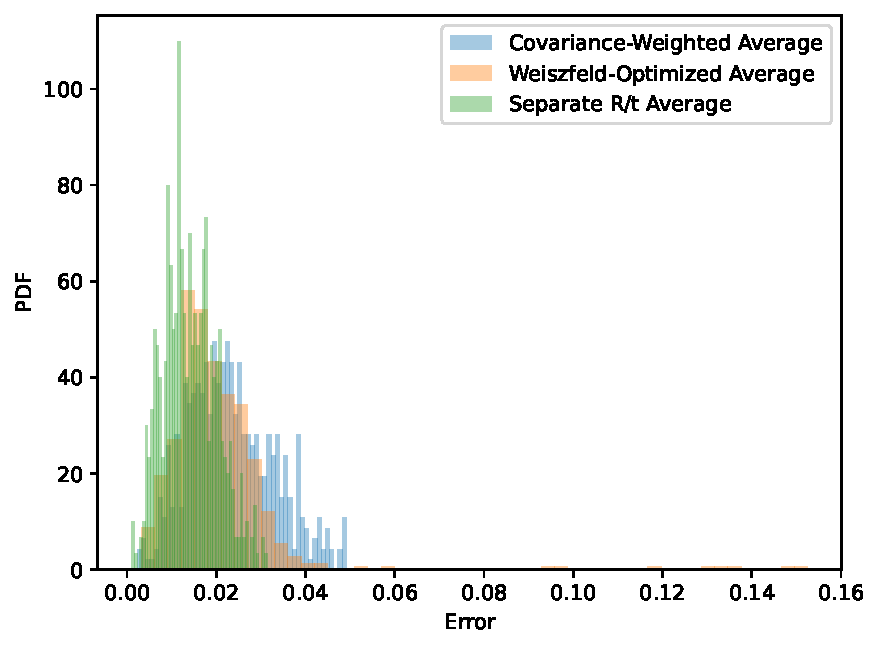
\includegraphics[width=0.46\linewidth]{images/pose_avg_trans.pdf}
	}
	\hspace{1pt}
	\subcaptionbox{Distribution of average rotation error.}{
		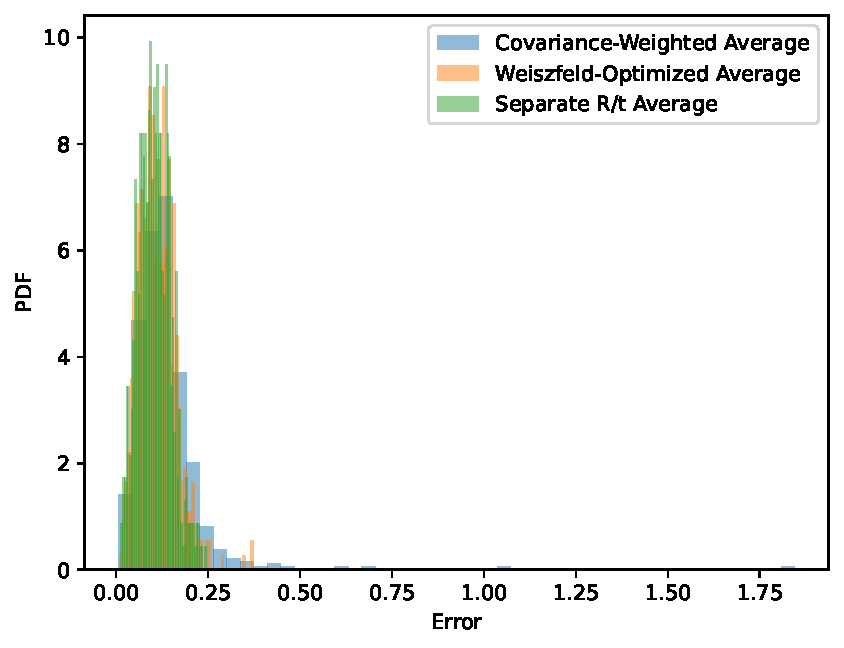
\includegraphics[width=0.45\linewidth]{images/pose_avg_rot.pdf}
	}
	\caption[Rotation and translation averaging experiment]{Comparing the behaviour of three different pose averaging techniques. We generate a random pose (expected mean), then sample 100 poses around it, by sampling a normal distribution of known $\sigma$ for each parameter.
		The sample poses are averaged using the target algorithm, and we compute a translation and a rotation error:
		$e(\tone, \ttwo) = \normtwo{\tone - \ttwo}$
		and
		$e(\Rone, \Rtwo)=\normtwo{\Logmap{\Rone^{-1}\Rtwo}}$,
		respectively.
	}
	\label{fig:pose-averaging}
\end{figure}

% First, we linearize $\pose$ around a constant pose $\pose_0$, with a perturbation $\xi \in \RR^6$:
% \begin{equation}
% 	\label{eq:poselin}
% 	\pose = \pose_0 \Expmap{\xi}
% 	\comma
% \end{equation}
% which leads to:
% \begin{align}
% 	\customres
% 	 & = \Log{\left(\pose_0 \Expmap{\xi}\right)^{-1} \Mtx{}} \\
% 	 & =	\Log{\Expmap{-\xi}\pose_0^{-1} \Mtx{}}               \\
% 	 & =  \Log{\pose_0^{-1} \Mtx{}} - \xi
% 	\eqdot
% \end{align}

% Next, we can derivate the $\mathcal{D}$ function with respect to $\xi$:
% \begin{align}
% 	\frac{\delta \mathcal{D}}{\delta\xi}
% 	 & = \frac{\delta \left(\transpose{\customreslin} \CovM^{-1} \customreslin\right)}{\delta\xi} \\
% 	 & = -\CovM^{-1}\customreslin
% 	\eqdot
% \end{align}

% The minimum of the cost function in Eq.~\ref{eq:costfn} occurs when:
% \begin{equation}
% 	\sum_{\Mtx{}} -\betaM \CovM^{-1}\customreslin = 0
% 	\comma
% \end{equation}
% which, when solved for $\xi$, gives:
% \begin{equation}
% 	\xi = \left(\sum_{\Mtx{}}\betaM\CovM^{-1}\right)^{-1}
% 	\sum_{\Mtx{}}\betaM\CovM^{-1}\customreslinnoxi
% 	\eqdot
% \end{equation}

% The final pose is reconstructed using the relationship in Eq.~\ref{eq:poselin}. We note that this procedure actually computes a weighted combination of poses --- both the covariance matrices and the $\betaM$ terms act as weights. For small covariance values, the contribution of the associated pose $\Mtx{}$ is large, because $\CovM$ is inverted. In practice, we found it convenient to only take into account the covariances, in order to avoid having to adjust the additional $\betaM$ terms, which scale the weights linearly.





% If $\xiicp$ and $\xigps$ are the twist vector residuals for registration and GPS costs respectively (we discard the motion prediction pose cost for simplicity, without loss of generality), the cost function becomes:
% \[
% 	\mathcal{J}\left(\pose\right) =
% 	\transpose{\xiicp} \cdot \covicp^{-1} \cdot \xiicp +
% 	\transpose{\xigps} \cdot \covgps^{-1} \cdot \xigps
% \]

\subsection{Motion prediction}
\label{subsec:motion-prediction}


The first component that we analyse addresses the problem of predicting the next pose in the trajectory. Given the trajectory computed so far $\left\{\pose_0, \pose_1, \dots \pose_t \right\}$, we are looking for $\pose_{t+1}'$ that estimates the location and orientation of scan $P_{t+1}$ in the world frame.

This influences two other elements of the framework: motion compensation and point cloud registration. In the absence of IMU data, the displacement between consecutive scans can be interpolated to correct individual points. Point cloud registration uses this predicted pose as an initial guess, for faster convergence, as we will see in a later section.

If the scans are captured at small, equal intervals, as is usually the case for LiDAR sensors, the movement can be approximated by a constant velocity model. The displacement between the previous two scans is propagated using
$\Delta \pose_{t}' \approx \Delta \pose_{t-1} = \pose_{t-1}^{-1}\pose_{t}$, which leads to
$\pose_{t+1}' = \pose_{t} \Delta \pose_{t-1}$. In our case, the time steps are not necessarily equal, and we would like to correct this pose estimate using the GPS measurements, when available, so we experimented with a Kalman Filter for computing the location component of $\pose_{t+1}'$. The state $\bm{x}_k \sim \mathcal{N}(\kfx{k}, \kfP{k}) $ is formulated as:
\begin{align}
	\kfx{k} & = \transpose{\left[x_k, y_k, z_k, {v_x}_k, {v_y}_k, {v_z}_k\right]}                                                \\
	\kfP{k} & = \text{diag}\left(\varx{x_k}, \varx{y_k}, \varx{z_k}, \varx{{v_x}_k}, \varx{{v_y}_k}, \varx{{v_z}_k}\right)\eqdot
\end{align}
Over a time step $\Delta t$, this changes according to a linear model:
\newcommand{\Fdt}{\matx{F}(\Delta t)}
\newcommand{\Qdt}{\matx{Q}(\Delta t)}
\begin{align}
	\kfxpred{k+1} & =  \Fdt \cdot \kfx{k}                              \\
	\kfPpred{k+1} & = \transpose{\Fdt} \cdot \kfP{k} \cdot \Fdt + \Qdt
	\comma
\end{align}
where
$
	\Fdt =
	\begin{bmatrix}
		\matx{I}_3 & \matx{I}_3 \Delta t \\
		\matx{0}_3 & \matx{I}_3
	\end{bmatrix}
$ and $\Qdt$ is the estimated process noise, which scales with the time interval. In the update step, we compute the new mean and covariance using a measurement $\bm{z}_k \sim \mathcal{N}(\vecx{z}_k, \matx{R})$, by applying a Kalman gain:
\begin{align}
	\matx{K}  & = \kfPpred{k+1} \matx{H} \left(\matx{H} \kfPpred{k+1} \transpose{\matx{H}} + \matx{R}\right)^{-1} \\
	\kfx{k+1} & = \kfxpred{k+1} + \matx{K} \left(\vecx{z}_k - \matx{H}\kfxpred{k} \right)                         \\
	\kfP{k+1} & = \left(\matx{I} - \matx{K} \matx{H}\right) \kfPpred{k+1}
	\eqdot
\end{align}

The $\vecx{z}_k$ vector consists of a location $\transpose{\left[x_\text{GPS}, y_\text{GPS}, z_\text{GPS}\right]}$ and velocity values $\frac{1}{\Delta t}\transpose{\left[x_\text{GPS} - x_k, y_\text{GPS} - y_k, z_\text{GPS} - z_k\right]}$, assuming linear displacement. The Jacobian $\matx{H}$ with respect to the state vector is $\matx{I}_6$, and the covariance of the measurement noise $\matx{R}$ can be estimated using the covariance of the GNSS reading. If no GNSS reading is associated with the current scan, the pose estimate is retrieved from the predicted position $\kfxpred{k+1}$, and the update step is performed based on the pose computed by the registration procedure.

This type of motion prediction method suffers from several disadvantages which outweigh its benefits for our use case. Firstly, it does not address the rotation component of the poses. Some possible workarounds include copying the orientation from the previous pose and letting the registration component correct that --- this has been observed to fail when a larger time gap occurs, especially for curved trajectories \reffigbr{reg-failure-rotation} ---, using the rotation returned by the INS, or having a separate method for computing the new rotation. Secondly, it introduces the need for reliable noise estimation \reffigbr{motion-model-overshoot}, such that the model is reactive to unexpected movement, while filtering out measurement noise. Process noise covariance $\matx{Q(\Delta t)}$ and the measurement input covariance $\matx{R}$ require approximations which are difficult to balance for a general solution. Therefore, using the estimated uncertainty of the predicted pose in further computations would only propagate potential sources of error.

% \begin{figure}[h]
% 	\centering
% 	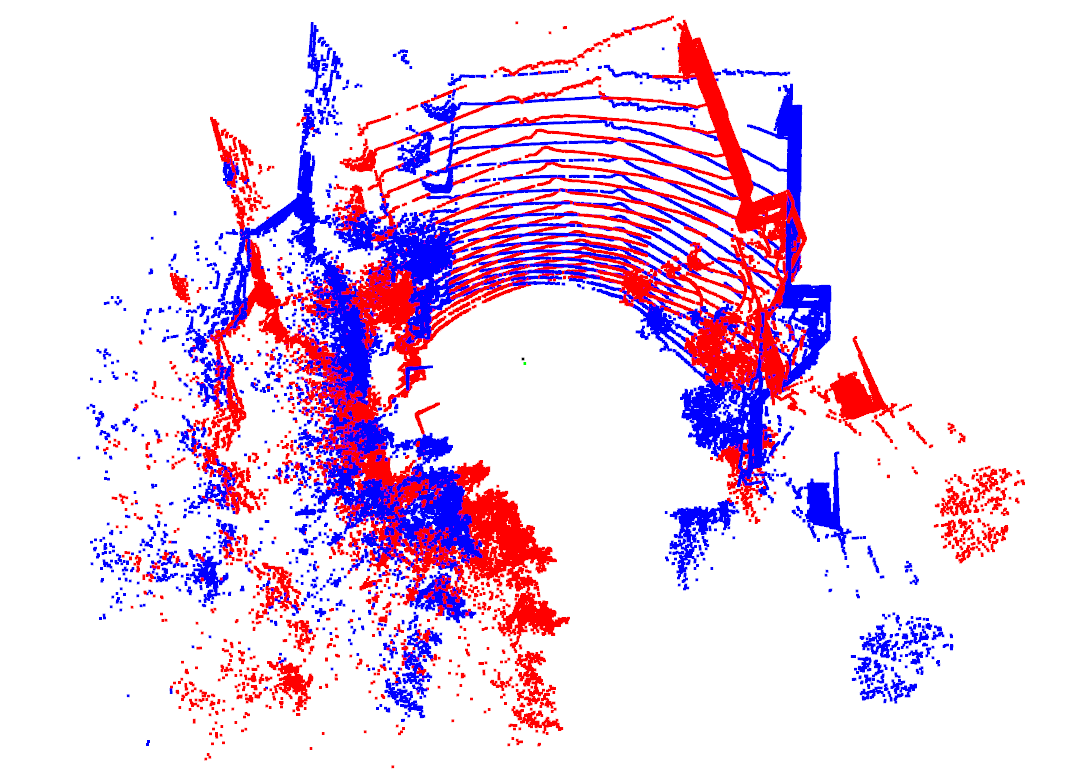
\includegraphics[width=0.5\linewidth]{images/rotation.png}
% 	\caption[Registration Failure Case (Rotation)]{Registration failure case.\\ Incorrectly estimating the rotation between scans (red and blue) can cause the registration to converge to an erroneous local minimum.}
% 	\label{fig:reg-failure-rotation}
% \end{figure}
\begin{figure}
	\centering
	\subcaptionbox{Registration failure case, when the rotation between consecutive scans (red and blue) is estimated incorrectly. The ICP algorithm converges to an erroneous local minimum. \label{fig:reg-failure-rotation}}{
		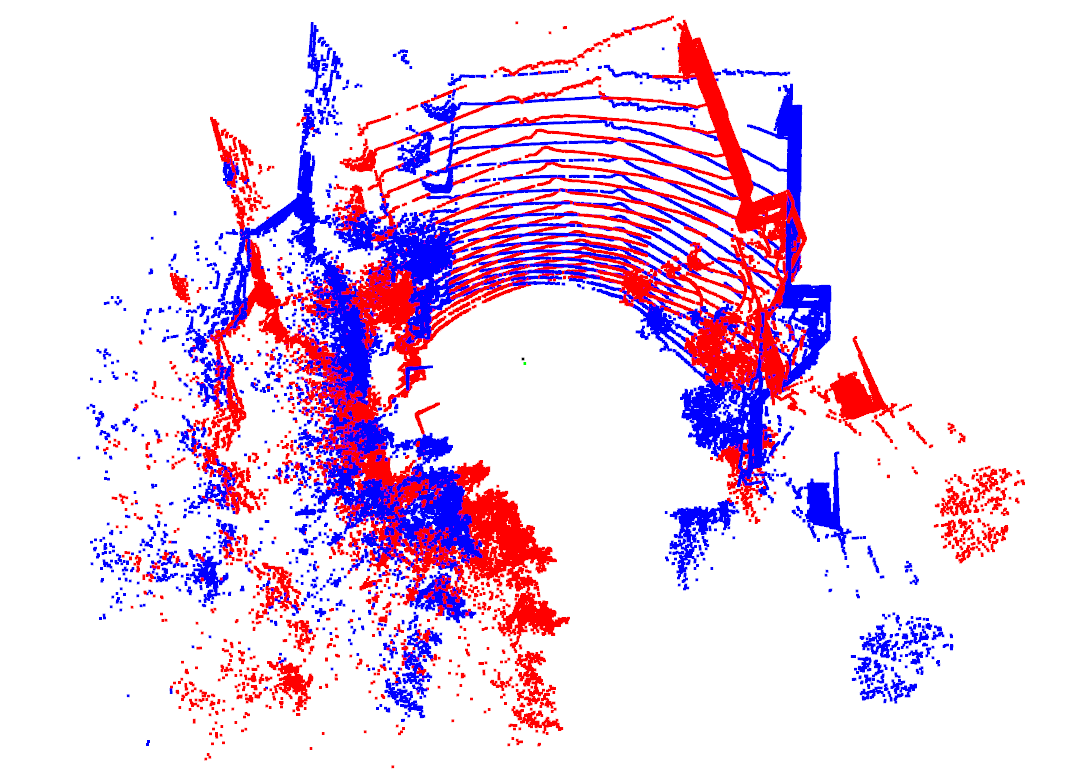
\includegraphics[width=0.47\linewidth]{images/rotation.png}
	}
	\hspace{1pt}
	\subcaptionbox{If the motion model is too confident in its velocity estimate, or uneven time intervals are not handled correctly, the motion prediction will overshoot. Trajectory starts from top right.\label{fig:motion-model-overshoot}}{
		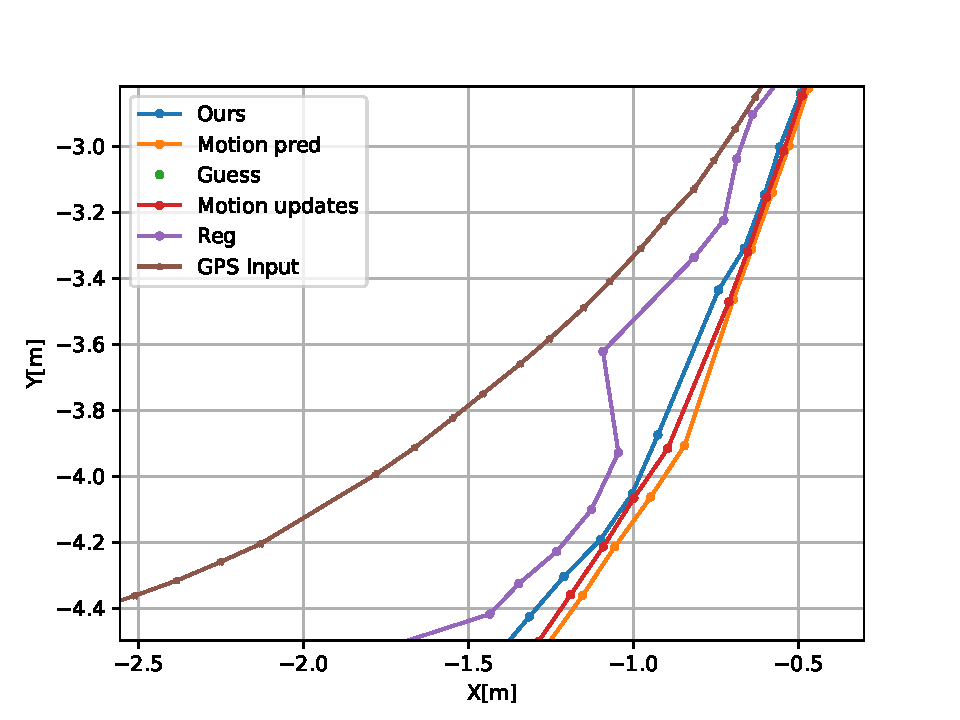
\includegraphics[width=0.47\linewidth]{images/motion-overshoot.pdf}
	}
	\caption[Motion model challenges]{Challenges of using a Kalman Filter motion model.}
	\label{fig:motion-pred-trouble}
\end{figure}


The approach that we propose relies on the interpolation properties of the $\SE{3}$ manifold (Eq.~\ref{eq:se3-interpolation}). In our case, using $\pose_{t-1}$ and $\pose_{t}$ to compute $\pose_{t+1}'$ is actually a matter of extrapolation, because we expect $\alpha$ to be approximately 2 at most steps, which would lead to unstable behaviour in the Lie group transformation. To avoid this, we first compute $\pose_{t+1}'' = \pose_{t}\pose_{t-1}^{-1}\pose_{t}$, and then obtain $\pose_{t+1}' = \varphi\left(\pose_t, \pose_{t+1}'', \alpha_{t}-1\right)$, where $\alpha_{t}= \frac{s_{t+1} - s_{t-1}}{s_t - s_{t-1}}$. For the scenarios that we have tested on, this provides a very good approximation of the correct displacement, which can be further refined using the information in the point cloud.

\subsection{Point Cloud Registration}
\label{subsec:registration}

The LiDAR sensor perceives the environment in a digital, discrete way, and outputs a set of 3D coordinates in the local frame. In a static scene, or after accurate motion compensation (Section~\ref{subsec:motion-compensation}), this represents a high-quality 3D snapshot of the environment from the current viewpoint. The mechanical design of the sensor introduces some particularities in the data \reffigbr{pcd-effects}, but the measurement accuracy is excellent. As described earlier, applying a noise-resilient registration algorithm between consecutive scans constitutes a sensible odometry estimate.

\begin{figure}
	\centering
	\subcaptionbox{The circular pattern on the ground section is typical for rotating LiDARs. Point density decreases with distance and incidence angle.}{
		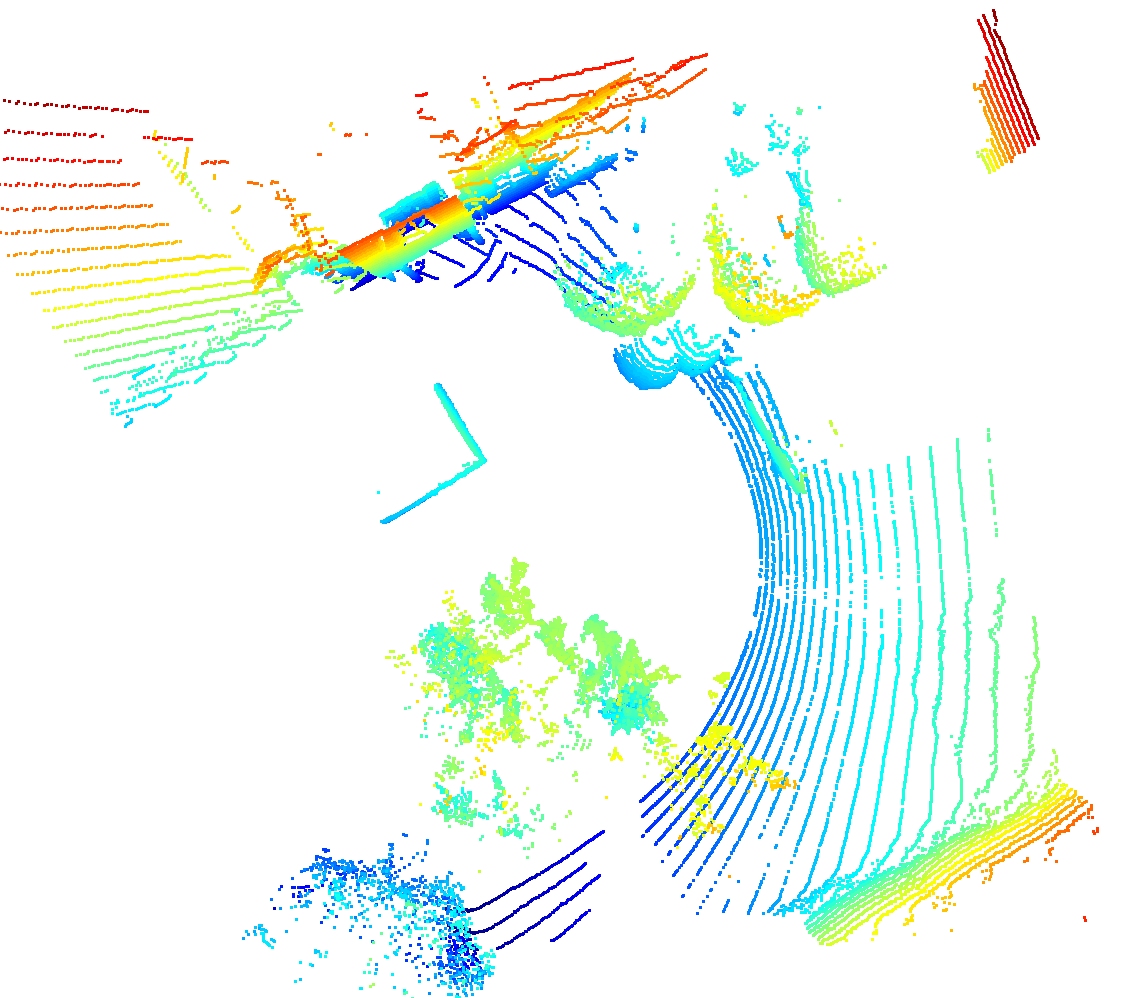
\includegraphics[width=0.47\linewidth]{images/pcd-circles.png}
	}
	\hfill
	\subcaptionbox{Laser rays cannot penetrate opaque surfaces. This results in a ``shadow'' effect --- no points are generated for objects that are occluded from the sensor viewpoint.}{
		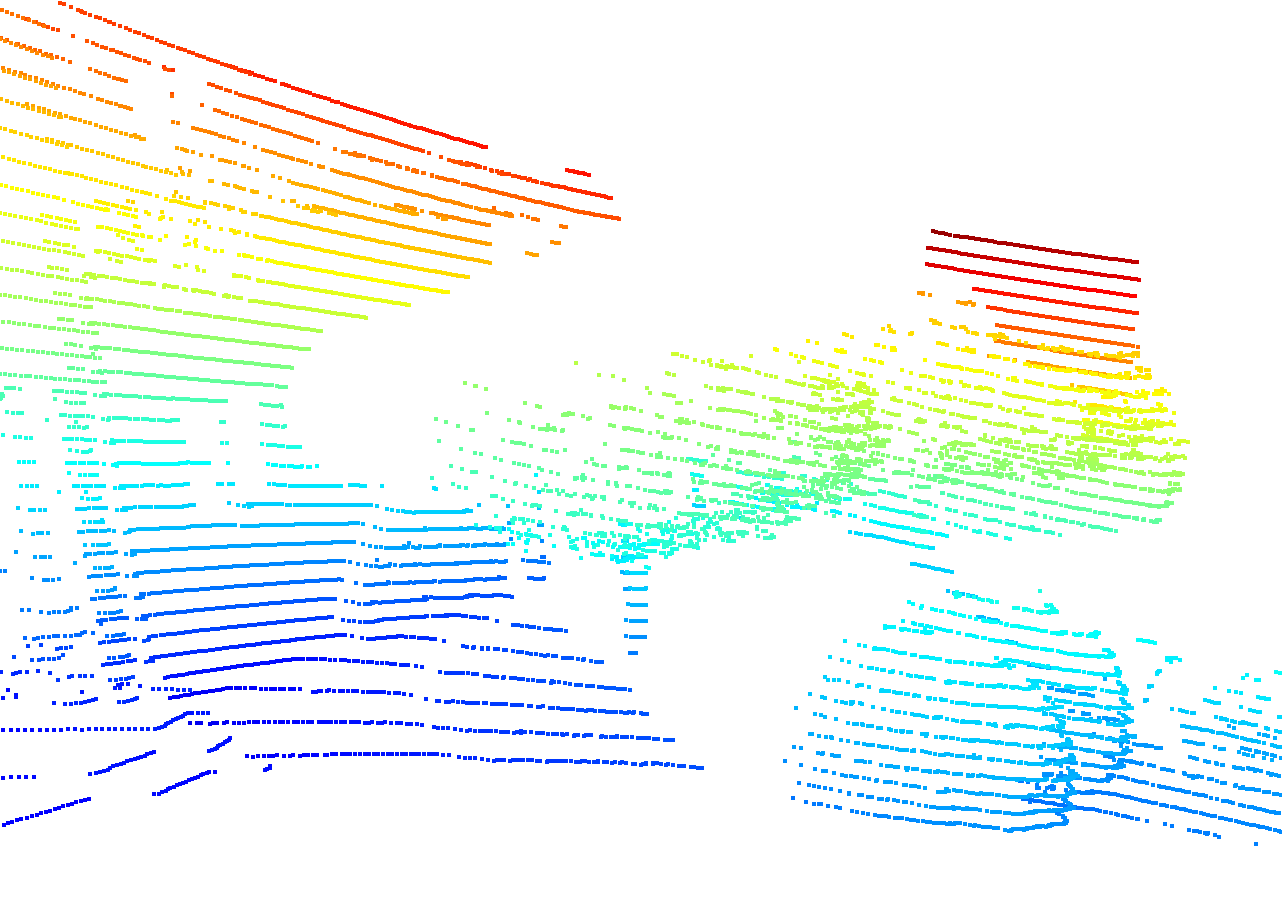
\includegraphics[width=0.48\linewidth]{images/pcd-shadows.png}
	}
	\caption[Particularities of LiDAR output]{Particularities of LiDAR output.}
	\label{fig:pcd-effects}
\end{figure}

\subsubsection{The ICP algorithm}
\newcommand{\pointp}{\vecx{p}}
\newcommand{\pointq}{\vecx{q}}
\newcommand{\matR}{\matx{R}}
\newcommand{\vect}{\vecx{t}}
\newcommand{\normalq}{\vecx{n}_{q}}
\newcommand{\covp}{\matx{C}_{p}}
\newcommand{\covq}{\matx{C}_{q}}
\newcommand{\distxpq}[1]{d_{#1}(\pointp, \pointq)}
\newcommand{\distpq}{\matR\pointp + \vect - \pointq}
\newcommand{\distpqi}{\matR\pointp_i + \vect - \pointq_i}
A baseline for \emph{fine} registration methods, Iterative Closest Point (\refalg{alg:pseudocode-icp}) is naturally applicable to our scenario, albeit with some modifications. As opposed to \emph{coarse} registration, where the aim is to find a rough alignment between arbitrary point clouds, we can exploit the motion prediction and/or the GPS readings as prior information about their global pose.

\newcommand{\distth}{d_\text{max}}
\newcommand{\tguess}{\matx{T}_\text{init}}
\begin{algorithm}
	\caption[Pseudocode of the point-to-point ICP algorithm.]{Pseudocode of the point-to-point ICP algorithm.}
	\label{alg:pseudocode-icp}

	\textbf{Input:}
	\begin{compactitem}
		\item $P, Q$: two point clouds, in local coordinate frames
		\item $\tguess$: initial transformation guess between $P$ and $Q$
		\item $\distth$: upper distance threshold for point neighbor search
		\item $\iterth$: upper iteration threshold for the algorithm
	\end{compactitem}
	\textbf{Output:}
	\begin{compactitem}
		\item $\pose$: registration pose between $P$ and $Q$
	\end{compactitem}
	\textbf{\underline{Funct}} ICP($P, Q, \tguess, \distth, \iterth$)
	\begin{algorithmic}[1] % number every line
		\State $\pose \leftarrow \tguess$
		\State $P' \leftarrow P$ transformed with $\pose$
		\For{$i=1, \dots, \iterth$}
		\State Compute nearest-neighbor correspondences between $P'$ and $Q$
		\State Discard correspondences where $\normtwo{p' - q} > \distth$
		\State Compute $\pose' \leftarrow  \underset{\pose}{\text{argmin}} \sum_{p', q}\normtwo{\pose \begin{bmatrix}
					p' \\1
				\end{bmatrix}  - \begin{bmatrix}q \\ 1\end{bmatrix}}$
		\State $\pose \leftarrow \pose'\pose$ \Comment{Update the transformation estimate}
		\State $P' \leftarrow P'$ transformed with $\pose'$ \Comment{Update the point cloud}
		\EndFor
		\State \textbf{return} $\pose$
	\end{algorithmic}
\end{algorithm}

At every iteration step, the algorithm generates a set of correspondence hypotheses --- a heuristic approximation of true correspondences --- by finding the closest point from $Q$ to each point in $P'$. The assumption is that the alignment of the two point clouds is improved by minimizing the distance associated with each correspondence. Depending on how the distance metric is defined, the algorithm can focus on different characteristics of the point clouds. The simplest formulation uses a point-to-point distance metric.
Given a transformation estimate $\pose = \left(\matR, \vect\right)$, we have:

\begin{equation}
	\distxpq{1} = \normtwo{\distpq}
	\eqdot
\end{equation}
This is a computationally-efficient approach, but is more sensitive to noise and outliers compared to the alternatives, and it does not take into account any geometrical features of the point clouds. To improve this, a point-to-plane metric \cite{chen1991pointtoplane} can be used, which considers the unit surface normal $\normalq$ computed at $\pointq$:

\begin{equation}
	\distxpq{2} = \left(\transpose{\normalq}\left(\distpq\right)\right)^2
	\eqdot
\end{equation}
Because $d_{2}(\pointp, \pointq)$ is null when $\pointp$ lies on the plane defined by $\pointq$ and $\normalq$, this approach improves surface registration, but will struggle in unstructured environments where the normals cannot be reliably estimated. In general, this is achieved by considering the neighborhood of each point in $Q$, fitting a plane to it, and computing its normal.

In a more general formulation, the local surface properties are captured by the covariance matrices $\covp, \covq$ computed at $\pointp$ and $\pointq$ respectively. The resulting distance metric \cite{segal2009generalized} is:

\begin{equation}
	\distxpq{3} =
	\transpose{\left(\distpq\right)}
	\left(
	\matR \covp \transpose{\matR} + \covq
	\right)^{-1}
	\left(\distpq\right)
	\eqdot
\end{equation}

All of the above can constitute the residual terms when computing the optimal transformation using a Least-Squares solver. To improve noise robustness, several additional techniques are employed. We prevent the creation of correspondences beyond a given distance threshold, to avoid introducing incorrect point pairs. Using a small threshold, however, causes the algorithm to converge to a local minimum, as it is unable to correct for larger displacements (\eg when the initial transformation guess is far from the optimum). Inspired by \emph{Trimmed ICP} \cite{trimmedicp}, we sort correspondences by distance and discard those that are above the 70th percentile, under the assumption that the majority of pairs will provide sufficient information for a satisfactory alignment.

\begin{figure}
	\centering
	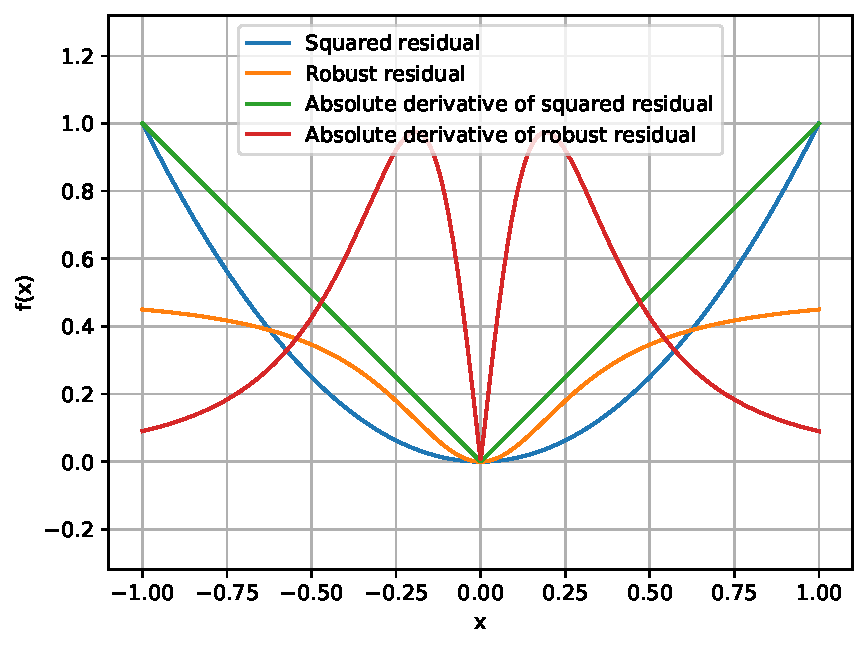
\includegraphics[width=0.5\linewidth]{images/robust-fn.pdf}
	\caption[Robust residual function]{Applying the Geman-McClure function ($\kappa=0.11$) to the correspondence residuals modifies their relative contribution during least-squares optimization, potentially improving convergence.}
	\label{fig:robust-residual}
\end{figure}
\newcommand{\residuali}{\vecx{r}_{i}}
\newcommand{\residualjac}{\matx{J}_{\residuali}}
Moreover, we apply the Geman-McClure function \reffigbr{robust-residual} on the point-to-point distance metric, like in \cite{vizzo2023ral}, which diminishes the influence of large residuals during minimization. For a residual $r$, this is defined as:
\begin{equation}
	\rho(r) = \frac{r^2/2}{\kappa + r^2}
	\comma
\end{equation}
where $\kappa$ is a custom scaling factor, set to 0.11 in our experiments. The optimization problem becomes:

\begin{equation}
	\pose^* = \underset{\pose}{\text{argmin}} \sum_{i}
	\rho \left(\normtwo{\distpqi} \right)
	\comma
\end{equation}
which can be solved using the Gauss-Newton algorithm. We parametrize $\pose$ as a twist vector $\xi \in \RR^6 $ and we linearize around $\matx{I}_4$, to obtain $\pose \approx \matx{I}_4 + \xihat$. The Jacobian of the residual $\residuali =\distpqi$ with respect to $\xi$ is:

\begin{equation}
	\residualjac = \begin{bmatrix}
		\matx{I}_3 & -\widehat{\vecx{t}}
	\end{bmatrix} \in \RR^{3\times6}
	\comma
\end{equation}
and each correspondence is associated a weight, according to the robust kernel:

\begin{equation}
	w(\residuali)=\frac{\kappa^2}{(\kappa + \normtwo{\residuali}^2)^2}
	\eqdot
\end{equation}
The resulting normal equation is:
\begin{equation}
	\sum_{i} w(\residuali)\transpose{\residualjac}\residualjac\xi =
	\sum_{i} w(\residuali)\transpose{\residualjac}\residuali
	\comma
\end{equation}
which can be rewritten as a conventional matrix equation $	\matx{A}\xi = \vecx{b}$. This can be solved in several ways, but we selected the Cholesky factorization method, thanks to its numerical stability. The wanted transformation is then retrieved as $\pose = \Expmap{\xi}$.

\subsubsection{Point Cloud Filtering}

We have also experimented with approaches that decrease the size of the point clouds used for registration. This is desirable because it reduces processing time and has the potential to remove points that skew registration results, such as those originating from regions occupied by trees or bushes. These regions are usually not sparse, so filtering based on the distance to the nearest neighbor or a related statistical measure was not very effective.
Similarly, random downsampling is not effective, because it does not address the noise issues.

A promising method was based on the formulation described in \cite{adolfsson2021coral}, which computes a per-point entropy measure using the covariance of its neighborhood.
A low entropy value indicates a structured, well-formed region (\eg points on a planar surface), while high entropy is usually associated with noisy regions. \reffigbr{sub-entr-view}
The size of the neighborhood, defined as a radius around each point, was set to 0.3m.
Filtering discards points with entropy above a certain percentile, to avoid setting a fixed threshold that would not be able to adjust to variable scene features. \reffigbr{sub-entr-log} Unfortunately, this is computationally expensive and does not visibly improve registration results.

\begin{figure}
	\centering
	\subcaptionbox{Entropy values in a scene with plenty of vegetation. Red - high entropy, green - low entropy. For covariance estimation, the neighborhood radius is 0.3m. \label{fig:sub-entr-view}}{
		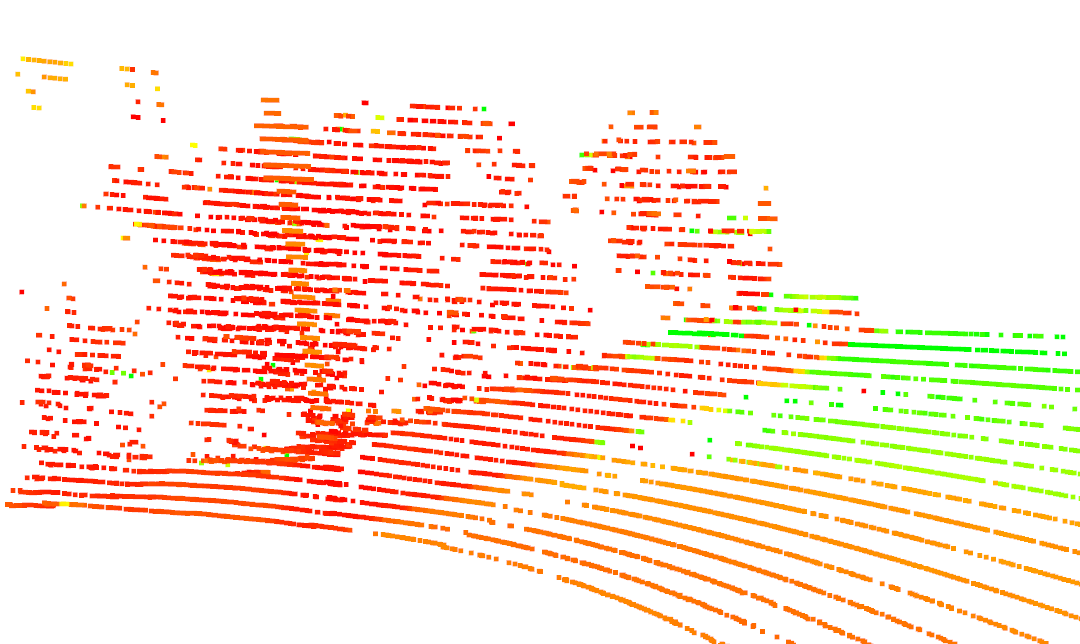
\includegraphics[width=0.47\linewidth]{images/entropy-scan.png}
	}
	\hfill
	\subcaptionbox{Per-scan entropy across a section of the dataset. Entropy values vary depending on the scene features, making it difficult to find a satisfactory global threshold.\label{fig:sub-entr-log}}{
		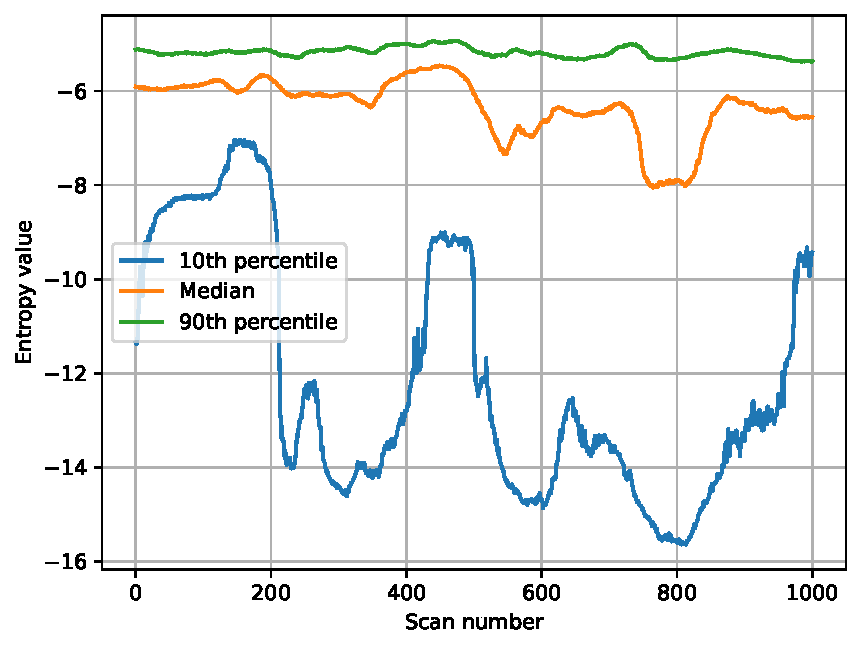
\includegraphics[width=0.48\linewidth]{images/entropy-log.pdf}
	}
	\caption[Filtering using entropy]{Point Cloud entropy analysis.}
	\label{fig:entropy-analysis}
\end{figure}

More advanced techniques involve finding salient points or structures that can be identified in multiple scans (also referred to as \emph{landmarks}, in the SLAM paradigm), either through feature extraction \cite{fpfh} or 3D segmentation, but this introduces a map representation that is not really applicable to our use case.

We employ a voxelization mechanism similar to \cite{vizzo2023ral}, to balance computation time and noise robustness. The 3D space is divided into equal-size cells and the first point in each cell is kept. The voxel size controls the resolution of the filtered point cloud, and should be smaller than the distance threshold used for correspondence generation, to avoid degenerate scenarios.

\subsubsection{Estimating Registration Covariance}
\newcommand{\degrad}[1]{\text{rad}(#1)}
A particular challenge is raised by the need to estimate the covariance of the pose obtained as the registration result. This serves as a confidence measure for the optimization framework, where the residuals are scaled with the inverse of $\covicp \in \RR^{6 \times 6}$.
Brossard et al. \cite{Brossard_2020} provided an in-depth analysis of this problem. Previous works have computed covariance based on the Jacobian involved in the correspondence distance minimization \cite{covarianceicp2} or by employing a Kalman Filter that is updated for each point, using the mean squared correspondence distances as a measurement noise estimate \cite{covarianceicp}.

We propose a heuristic approach based on the \acrfull{rmse} $e$ of the inlier correspondences in the registration result --- those for which the distance is below the provided threshold. Assuming that a perfect alignment corresponds to a covariance $\covicp^{*}$ with $\sigma_{x, y, z} = 0.01$ and $\sigma_{\phi, \theta, \psi} = 2\degree$,
we compute a factor:
\begin{equation}
	r = 1 + \text{max}\left(0, \frac{e-e_{\text{min}}}{\sigma_e}\right)
\end{equation}
and set $\covicp = r \cdot \covicp^{*}$. Here, $\sigma_e$ represents the standard deviation of the RMSE values computed so far, so $r$ is an indicator of how accurate the current registration is, relative to $e_{\text{min}}$, the smallest RMSE observed up to that point. We note that RMSE can sometimes be misleading (\eg when registration reaches a local minimum), but it provides a reasonable estimate of alignment quality in this context.

\subsubsection{Summary}

Following multiple experiments, we arrived at a procedure that can account for poor initialization and scene noise, while ensuring high-quality alignment between the current scan and the existing map. This is a two-step process, mimicking a coarse-to-fine registration procedure. Let $M, S$ be the map and current scan point clouds, respectively, and $v(P, \alpha)$ a voxelization function that downsamples point cloud $P$ using voxel size $\alpha$ (in meters). First, we perform robust point-to-point ICP between $v(S, 0.2)$ and $v(M, 0.4)$, using the motion prediction pose for initialization. The correspondence set is trimmed at the 70th percentile, and the number of iterations in the ICP procedure is not constrained, but we halt when the norm of the estimated $\xi$ is below a small threshold ($10^{-4}$).

The resulting pose is used to intialize a dense registration stage: $v(S, 0.1)$ is aligned with $v(M, 0.1)$ using Generalized ICP, for at most 100 iterations. In both cases, we use a distance threshold of 0.5m, to account for corrections even in sparser areas of the point cloud (\eg at the edges).

\subsection{Map Handling}

Because high-quality mapping constitutes one of our primary goals, having a sensible map representation is a key component of the solution. We treat the map as a point cloud in the global frame, built by concatenating a sequence of scans after transforming them with the best pose estimate computed so far. We do not attempt to store a set of key points, as this does not contribute to fine registration, but we constrain the size of the point cloud that we operate on using a sliding window approach. At every step, only the last $k=5$ scans are considered. This straightforward method ensures temporal and spatial relevance: we do not store points that have been observed a long time in the past or points that are far away from the current location.

One drawback is that it hinders the implementation of a loop-closure mechanism, as there is no possibility to perform registration against older scans, but this is not a stringent problem, as the usage of GNSS readings prevents large localization drifts.

\subsection{Graph Optimization}
\label{subsec:graph-optimization}

\begin{figure}
	\centering
	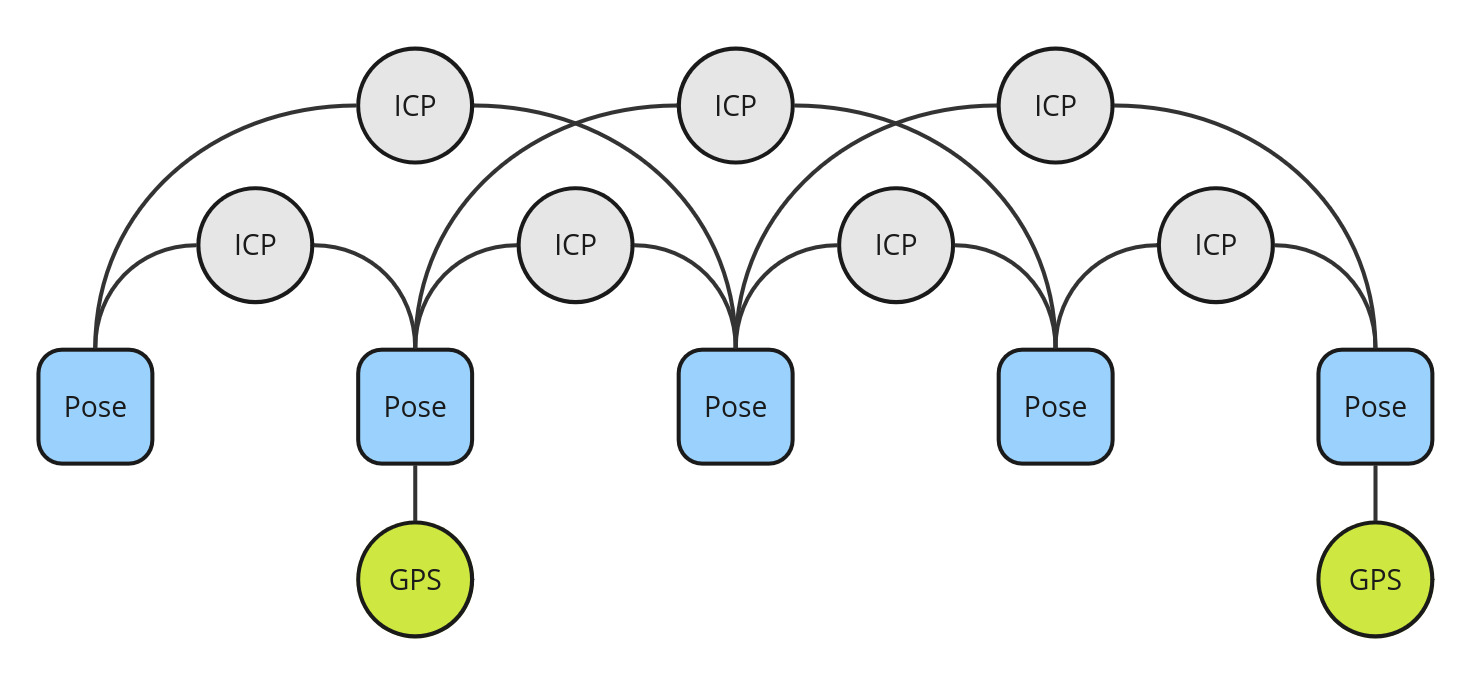
\includegraphics[width=0.6\linewidth]{images/graph.jpg}
	\caption[Factor Graph Structure]{The factor graph structure.\\If a GPS reading is available, a unary factor is created. The displacement predicted with point cloud registration (ICP) is used to create binary factors between consecutive poses, like a classical odometry factor. To achieve higher map quality, we also add ``skip connections'' based on the registration result.}
	\label{fig:factor-graph}
\end{figure}

As stated earlier, we also experimented with solutions that employ factor graph optimization, thanks to its natural affinity to the SLAM problem. A factor graph \cite{dellaert2012factor} is a bipartite graph where nodes represent either:
\begin{compactitem}
	\item variables --- these refer to variables in the problem domain; in our case, they are the estimated poses $\pose_i$ associated with each LiDAR scan, or
	\item factors --- probabilistic constraints, derived from measurements or prior information, whose residuals are to be minimized.
\end{compactitem}

\newcommand{\tigps}{\pose_i^{\text{GPS}}}
\newcommand{\tijicp}{\pose_{ij}^{\text{ICP}}}
\newcommand{\covigps}{\matx{\Sigma}_i^{\text{GPS}}}
\newcommand{\covijicp}{\matx{\Sigma}_{ij}^{\text{ICP}}}
In our problem, two types of factors are employed. The GPS readings $\left(\tigps, \covigps\right)$ introduce unary factors that constrain a single pose variable. The twist vector residual is:
\begin{equation}
	\vecx{r}_i^{\text{GPS}}\left(\pose_i\right) =
	\Logmap{\left(\tigps\right)^{-1}\pose_i}
	\eqdot
\end{equation}
Odometry measurements $\left(\tijicp, \covijicp\right)$ obtained from the point cloud registration create binary factors that are connected to the two pose variables between which the displacement occurred. The associated residual is:
\begin{equation}
	\vecx{r}_{ij}^{\text{ICP}}\left(\pose_i, \pose_j\right) =
	\Logmap{\left(\tijicp \right)^{-1} \left(\pose_i^{-1} \pose_j\right)}
	\eqdot
\end{equation}
If we define a covariance-scaled norm $
	\normm{\vecx{r}}_{\matx{\Sigma}}^2 =
	\transpose{\vecx{r}}\matx{\Sigma}^{-1}\vecx{r}
$ (note the similarity with Eq.~\ref{eq:mah-distance}), we can formulate the joint optimization problem:
\begin{equation}
	\mathfrak{T}^{*} = \underset{\mathfrak{T}}{\text{argmin}}
	\left(
	\sum_{i} \normm{\vecx{r}_i^{\text{GPS}}\left(\pose_i\right)}_{\covigps}^2
	+
	\sum_{i} \normm{\vecx{r}_{ij}^{\text{ICP}}\left(\pose_i, \pose_j\right)}_{\covijicp}^2
	\right)
	\eqdot
\end{equation}
In contrast with Section~\ref{subsec:reconciling}, this addresses the entire set of pose estimates, which is essential if trajectory corrections are to be applied retroactively and not just for the current pose.

The generic formulation of the registration pose residual $\vecx{r}_{ij}^{\text{ICP}}$ allows for a modification that improves overall map quality. At time step $k$, after aligning the current scan $P_k$ to the existing local map built from scans $\left\{P_{k-5}, \dots P_{k-1}\right\}$, we create two odometry factors, for $\left(\pose_{k-1},\pose_k\right)$ and $\left(\pose_{k-2},\pose_k\right)$. The latter is motivated by the early observation that a registration-only trajectory yields a high-quality 3D map, so we use an odometry factor to enforce the registration result not only between consecutive poses.
The final solution architecture, including the Factor Graph component, is presented in \reffig{solution-architecture}.
\begin{figure}[h]
	\centering
	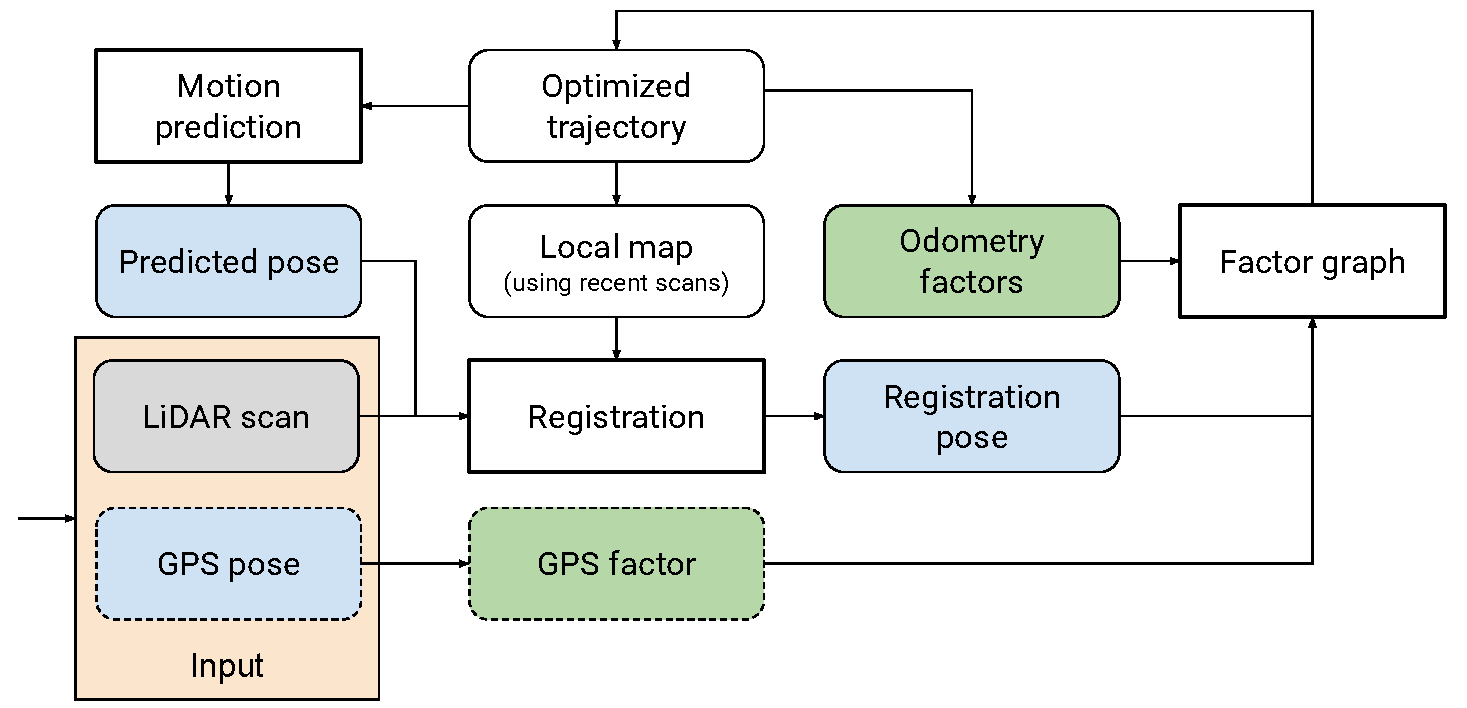
\includegraphics[width=0.7\linewidth]{images/solution-diagram.pdf}
	\caption[Solution Architecture]{Solution architecture and workflow.\\At each time step, the Factor Graph provides the best trajectory estimate using the information available so far. Registration is performed against a local map built from recent scans, using a motion-predicted pose as initial estimate. When a new pose is added to the graph, the registration result is used to create odometry factors that link it to previous poses. If a GPS pose is available, it introduces an additional factor.}
	\label{fig:solution-architecture}
\end{figure}

\section{Implementation details}

The experiments and framework described above have been implemented in \mbox{Python 3.8.10}~\cite{Python}, a high-level, interpreted programming language, which enabled fast development iterations.
We make intensive use of existing libraries for linear algebra operations (NumPy~\cite{harris2020array}, pytransform3d~\cite{Fabisch2019}) and point cloud processing (Open3D~\cite{Zhou2018}). We treat poses and point clouds as NumPy arrays of size $(4, 4)$ and $(n, 3)$, respectively. During the registration process, the nearest-neighbor search required for correspondence generation relies on the KD-tree data structure implemented in SciPy~\cite{2020SciPy-NMeth}. As we do not perform any modifications to the algorithm, we use the Generalized ICP implementation provided by Open3D. For factor graph operations, we chose the popular GTSAM~\cite{gtsam} library, despite the limited documentation available for its Python bindings.

An important mention is reserved to the Numba~\cite{numba} compiler library, which enabled significant performance improvements for operations on large NumPy arrays. Performing motion compensation, for example, would not be possible in real-time (\ie processing several LiDAR scans per second) in pure Python, but the just-in-time compilation provided by the Numba decorators, combined with parallel processing, alleviate this problem.

The code is divided into modules that group similar functionality, and we followed Object-Oriented Programming principles loosely, by having classes for the main components (\eg Registration, Motion model, Graph optimization). For faster experimentation, the data structure presented in Section~\ref{sec:data-acquisition} is transformed into raw numerical form, stored on disk as \texttt{.npy} files, and re-loaded at runtime. Naturally, some custom interfacing would have to occur in order to apply the current implementation for a live robotic system, but our particular use case did not raise the need for integration with the ROS~\cite{ros2009} framework.

